\onlyinsubfile{\setcounter{section}{2}}

\section{Data}
\label{sec:data}

\par For the statistical analysis in this paper, I use the RAND Longitudinal version of the Household Retirement Survey (HRS) for the years 2002-2022. First, I define asset classes and portfolios, which will be guided by the unique structure of the HRS data set. Then, I provide descriptive statistics on the underlying return components, as well as returns by asset and portfolio. From there, I discuss some statistics on the demographic variables which form the set of control variables in the regression models. Finally, I look at the relationship between returns to net wealth and a number of variables (net wealth, age, education, trust) and describe portfolio compositions across respondents.

\subsection{Sample restrictions}
\label{ssec:sample-restrictions}

\par After merging the RAND longitudinal extract with the constructed return and wealth fields, the analysis-ready wide file contains about 45{,}200 respondent identifiers; reshaping to a long person--year panel yields about 543{,}000 rows spanning the interview years used here. Most core RAND covariates are observed for a large share of those rows, but the key sample of interest is comprised of the respondents who have nonmissing values for the trust and returns to net wealth variables (along with the other variables used in the regression analysis). Wave-specific returns to net wealth (5\% winsorized within survey year) are nonmissing for about 137{,}000 person-years: many observations drop out in a given wave when wealth, flows, or other return ingredients are incomplete. Generalized trust is measured only in the 2020 module; in the long panel, 900 respondents have a nonmissing 2020 trust response, and that value is carried on their other waves so that about 10{,}800 person-year rows carry nonmissing trust for estimation.

\par The descriptive statistics for which observations are pooled (histograms, bin-scatter figures, return-by-age and return-by-education tables, and the portfolio composition tables below) restrict person-years to the same listwise-complete sample as a benchmark pooled OLS of 5\% winsorized returns to net wealth on quadratic trust with the baseline time-varying controls and education categories only---2{,}919 person-years. Of those, 449 rows are 2020 interviews and enter the trust histogram and the race-by-trust summary (all 449 have nonmissing generalized trust). The main regression tables in Section~\ref{sec:chapter2-results} use the specifications printed there (larger or smaller $N$ by column); the extended Correlated Random Effects (CRE) model for net wealth uses about 2{,}900 person-years. When the dissertation build sets a single unified Chapter~2 sample (extended CRE person-years), the corresponding flag yields about 2{,}900 person-years for tables and figures tied to that mode.

\subsection{Asset classes and portfolio definitions}

\par The HRS asks a number of questions aimed at measuring household wealth and portfolio composition in the sample. I collect data on:
\begin{enumerate}
  \item \textbf{Interest income and dividends}
  \item \textbf{Capital gains}
  \item \textbf{Net investment flows}
  \item \textbf{Wealth holdings of the previous period}
\end{enumerate}
All of which are required to define the desired measure of household returns. Since population-level administration data on these objects for individual taxpayers are not available in the United States, it is important to understand each component needed in the return calculation. This will help to determine whether or not our measured distribution of returns in this dataset is sensible. To understand what portfolios are accruing returns, we will let the structure of the HRS questions guide how we define returns to specific asset classes for which the survey collects data. From there, portfolios are defined as collections of these defined asset classes.


\subsubsection{Interest income and dividends}
\label{sssec:interest_income_dividends}

\par The HRS RAND product has a distinct way of measuring the interest income and dividends received on the main asset classes, such as stocks and bonds, private business and real estate. In particular, there is a variable (\texttt{HwICAP}) in the survey that measures \texttt{Household Capital Income}:

\begin{itemize}
  \item ``$\ldots$is the sum of household capital income received over the last calendar year, including business or farm income, self-employment earnings, gross rent, dividend and interest income, trust funds or royalties, and other asset income.''
  \end{itemize}

  \par This particular feature of the data drives the main modeling assumptions of this paper regarding measuring returns: \textit{asset classes are defined as narrowly as they can be given observation of interest income and dividends on those assets}. For example, although we see capital gains for stocks, business, bonds, and real estate, we do not observe interest income or dividends on these assets individually. Thus, returns to the narrowest asset class defined in this paper will be called \textbf{returns to core assets} and will consist of these assets.

  \par The RAND product has variables (\texttt{RwIPENA}) and (\texttt{RwISRET}) which measure \texttt{Individual Income from Employer from Pension or Annuity} and \texttt{Individual Income from Social Security Retirement}, respectively. Together, these describe the interest income and dividends on retirement assets, so a measure of \textbf{returns to retirement assets} can be constructed. Moreover, I define the first broader notion of portfolio returns by considering \textbf{returns to core and retirement assets}.

  \par A key assumption is that there are \textit{no interest income or dividends earned on residential assets}.\footnote{An assumption made after verifying that there is no ``interest income and dividends'' variable equivalent for the real estate asset class in the HRS dataset. } With this assumption, we can define \textbf{returns to residential assets}. 
  
  \par This accounts for the interest income and dividends for every variable that accrues some capital gains: either their interest income goes to core assets, retirement assets, or residential assets. Thus, interest income and dividends on the entire portfolio of assets (i.e. on net wealth) is the same as interest income and dividends on the portfolio with just core and retirement assets. \textbf{Returns to net wealth} are computed by adding the remaining available capital gains (and other components) for those variables that receive no interest income. For example, returns to net wealth includes capital gains for the \texttt{Net value of vehicles} (\texttt{HwATRAN}) and the \texttt{Net value of all other savings} (\texttt{HwAOTHR}), although these variables earn no interest income and dividends. The capital gains to the \texttt{Net value of businesses} (\texttt{HwABSNS}), on the other hand, show up both in the returns to core assets and returns to net wealth.

\par Figure~\ref{fig:interest_income_mean_by_year} shows the evolution of interest income and dividends over time within the relevant asset classes and for the overall portfolio.

\begin{figure}[H]
\centering
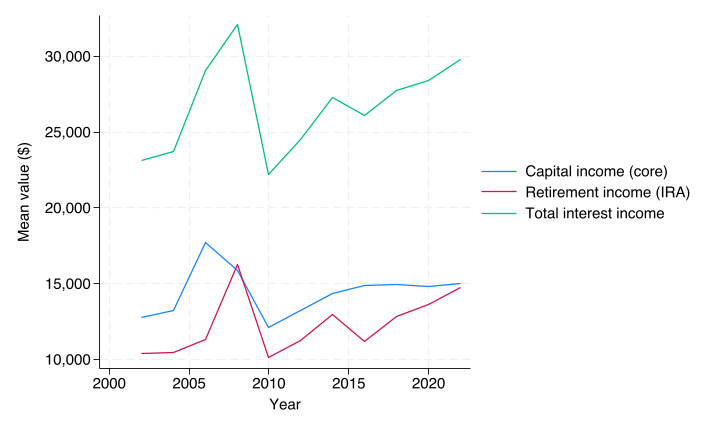
\includegraphics[width=0.8\textwidth]{../../Code/Descriptive/Figures/interest_income_mean_by_year.png}
\caption{Average interest income across respondents}
\label{fig:interest_income_mean_by_year}
\end{figure}
\FloatBarrier

\subsubsection{Capital gains}

\par Possible assets for which capital gains can be computed in the HRS are:
\begin{enumerate}
  \item \texttt{Net value of primary residences} (\texttt{HwATOTH})
  \item \texttt{Net value of secondary residences} (\texttt{HwANETHB})
  \item \texttt{Net value of real estate (not primary residence)} (\texttt{HwARLES})
  \item \texttt{Net value of business} (\texttt{HwABSNS})
  \item \texttt{Net value of IRA, Keogh accounts} (\texttt{HwAIRA})
  \item \texttt{Net value of stocks, mutual funds, and investment trusts} (\texttt{HwASTCK})
  \item \texttt{Net value of bonds and bond funds} (\texttt{HwABOND})
  \item \texttt{Net value of checking, savings, or money market accounts} (\texttt{HwACHCK})
  \item \texttt{Net value of CD, government savings bonds, and T-bills} (\texttt{HwACD})
  \item \texttt{Net value vehicles} (\texttt{HwATRAN})
  \item \texttt{Net value of other savings} (\texttt{HwAOTHR})
\end{enumerate}

\par Possible liabilities are:
\begin{enumerate}
  \item \texttt{Mortgage debt, primary residence} (\texttt{HwAMORT})
  \item Other \texttt{home loans} (\texttt{HwAHMLN})
  \item \texttt{Total other debt} (\texttt{HwADEBT})
\end{enumerate}

\par Capital gains for each asset is calculated as the estimated change in valuation across survey waves. Figure~\ref{fig:cg_core_assets_panels} shows the mean (blue) and median (red) for each wave of the survey for each possible asset.  

\begin{figure}[H]
\centering
\begin{minipage}[t]{0.48\textwidth}
\centering
\small\textbf{Private business}\par\vspace{0.25em}
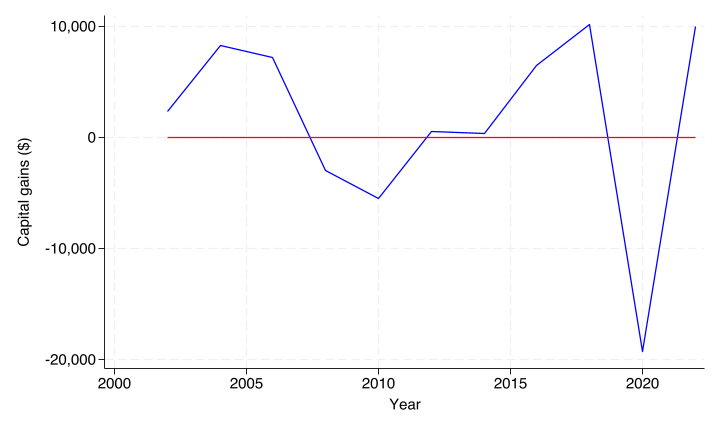
\includegraphics[width=\textwidth]{../../Code/Descriptive/Figures/cg_bus_mean_median_by_year.png}
\end{minipage}\hfill
\begin{minipage}[t]{0.48\textwidth}
\centering
\small\textbf{Stocks and mutual funds}\par\vspace{0.25em}
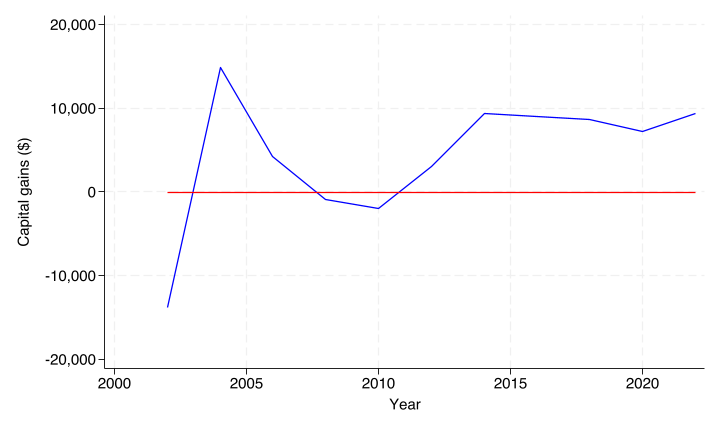
\includegraphics[width=\textwidth]{../../Code/Descriptive/Figures/cg_stk_mean_median_by_year.png}
\end{minipage}
\vspace{0.6em}
\begin{minipage}[t]{0.48\textwidth}
\centering
\small\textbf{Safe assets}\par\vspace{0.25em}
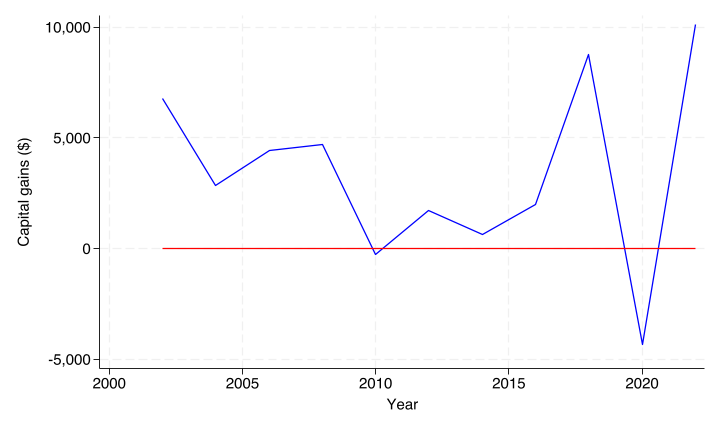
\includegraphics[width=\textwidth]{../../Code/Descriptive/Figures/cg_safe_mean_median_by_year.png}
\end{minipage}\hfill
\begin{minipage}[t]{0.48\textwidth}
\centering
\small\textbf{Other real estate}\par\vspace{0.25em}
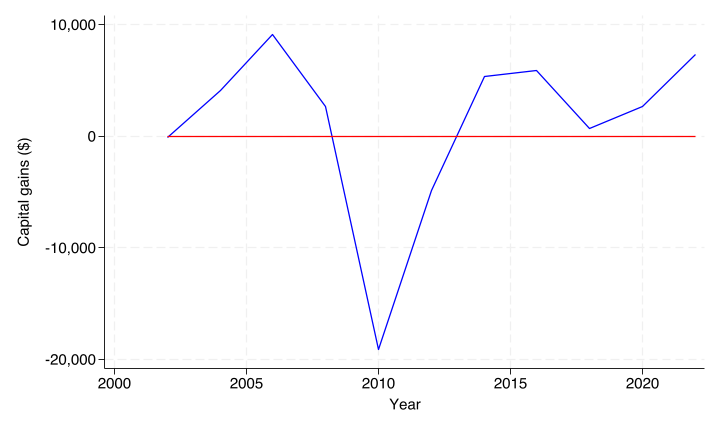
\includegraphics[width=\textwidth]{../../Code/Descriptive/Figures/cg_re_mean_median_by_year.png}
\end{minipage}
\caption{Capital gains in core assets}
\label{fig:cg_core_assets_panels}
\end{figure}

\par The \texttt{Net value of business} and \texttt{Net value of safe assets} each show a large decrease in average capital gains across respondents in the 2020 wave of the survey, likely an indication of the effects of the COVID-19 pandemic. The \texttt{Net value of real estate (not primary residence)} shows a similar decline in mean capital gains but in the 2010 wave of the survey, likely an indication of the effects of the Global Financial Crisis in 2008. Interestingly, \texttt{Net value of stocks, mutual funds, and investment trusts} shows no significant fall in average capital gains; notably, they begin at less than $-\$10{,}000$ and finish at around $\$10{,}000$ by the final wave of the survey. The \texttt{Net value of IRA, Keogh accounts} also starts out negative but ends well above $\$20{,}000$.

\FloatBarrier

\begin{figure}[H]
\centering
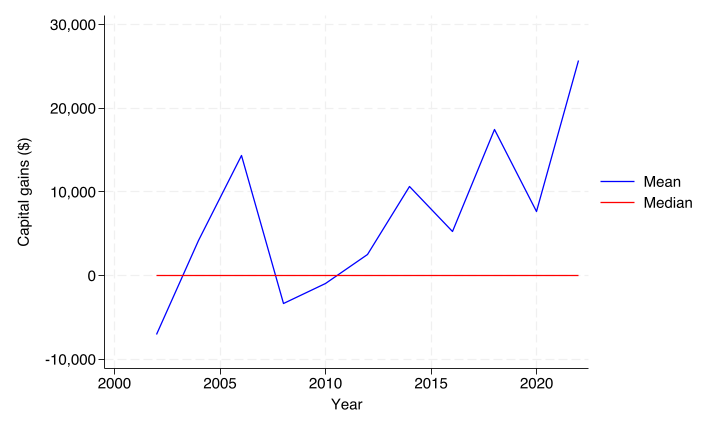
\includegraphics[width=0.8\textwidth]{../../Code/Descriptive/Figures/cg_ira_mean_median_by_year.png}
\caption{Capital gains in retirement assets}
\label{fig:cg_ira_by_year}
\end{figure}
\FloatBarrier

\par An important finding from inspecting the capital gains data is that most of the respondents do not have assets. This can be seen by the red median line at $0$ for most waves. This is another sign that the data are sensible so far -- a large amount of non-participation despite evidence of returns is consistent with the empirically documented equity premium puzzle: the inability to rationalize the excess premium return earned by risky assets over riskless assets.\footnote{See \cite{Mehra2003} for a review of this literature.}

\begin{figure}[H]
\centering
\begin{minipage}[t]{0.48\textwidth}
\centering
\small\textbf{Primary residence}\par\vspace{0.25em}
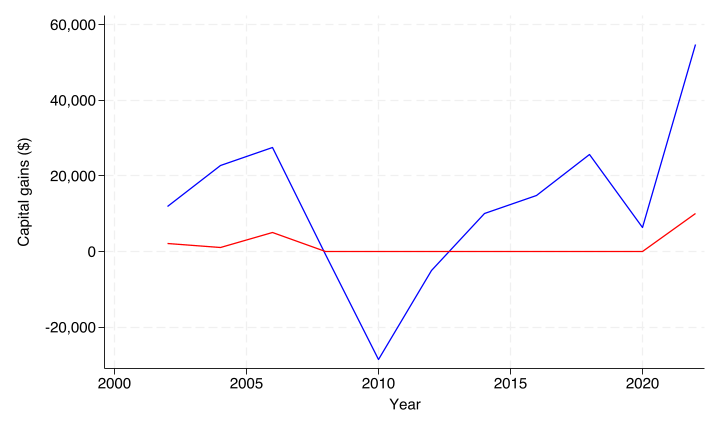
\includegraphics[width=\textwidth]{../../Code/Descriptive/Figures/cg_res_mean_median_by_year.png}
\end{minipage}\hfill
\begin{minipage}[t]{0.48\textwidth}
\centering
\small\textbf{Secondary residence}\par\vspace{0.25em}
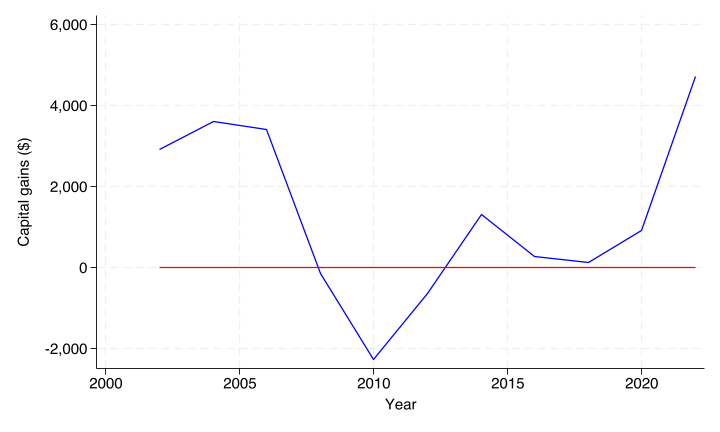
\includegraphics[width=\textwidth]{../../Code/Descriptive/Figures/cg_res2_mean_median_by_year.png}
\end{minipage}
\caption{Capital gains in residential assets}
\label{fig:cg_residential_panels}
\end{figure}
\FloatBarrier

\par Notably, the residential panel (Figure~\ref{fig:cg_residential_panels}) highlights that the mean of \texttt{Net value of primary residences} is much higher in level and volatility than the other assets, and is the only series with a clearly positive median in some years. The synchronized dip around 2008--2010 for the housing-related assets is another good sign regarding how reliably measured the data is.

%%%%%%%

\subsubsection{Net investment flows}

\par Net investment flows are vital in accurately computing returns because capital gains and interest income can miss other flows of value in a given asset class. Using the definitions of interest income and dividends from Subsubsection~\ref{sssec:interest_income_dividends}, I use these flows to construct net investment flows into three asset classes and two constructed portfolios:

\begin{enumerate}
  \item \textbf{Core assets}
  \item \textbf{Retirement assets}
  \item \textbf{Residential assets}
  \item \textbf{Core and residential assets}
  \item \textbf{Net wealth}
\end{enumerate}

\par An important concern regarding the RAND HRS Longitudinal product is that \textit{net investment flows are the only variables relevant to the calculation of returns that are not offered as cleaned and processed fields}. Instead, the net investment flow data for each asset must be merged in using the \href{https://hrsdata.isr.umich.edu/data-products/rand}{RAND HRS Fat File} for each survey wave. For this reason, there are substantially fewer observations for these variables by asset class than for the other return components. 

\par To resolve this issue, I do two things. First, I process the net investment flow variables per asset class myself using the associated Section~R flag for each amount. For example, \texttt{Personal funds into business amount} (\texttt{wR050}) and \texttt{Private business selling price amount} (\texttt{wR055}) pair with \texttt{Personal funds into business} (\texttt{wR049}) and \texttt{Sell any part interest in private business} (\texttt{wR054}), respectively; for primary and second homes, purchase and sale amounts (\texttt{wR007}, \texttt{wR013}) pair with \texttt{wR002}, and major improvement spending (\texttt{wR024}) pairs with \texttt{wR023}. When the gate item is ``no'' (\texttt{5}), the corresponding missing amount is set to zero. 


\par For the second step in handling missing values for net investment flows in a given asset class, retirement assets provide a useful example. In each wave, the HRS has three separate variables for net investment flows into IRA/Keogh accounts (\texttt{wQ171\_1}, \texttt{wQ171\_2}, and \texttt{wQ171\_3}). After using the accompanying flag variables (\texttt{wQ170\_1}, \texttt{wQ170\_2}, and \texttt{wQ170\_3}) to set some missing amount variables to zero, I define the \textbf{net investment flow for retirement assets} as the sum of these three components. So, if only one or two of the three retirement flow variables are observed, the retirement flow is simply the sum of the nonmissing components and it remains missing only if all three retirement flow variables are missing. 

\par Recall that net investment flows for business, stocks, and other real estate assets are combined into a \textbf{net investment flow for core assets}. The relevant net investment flow variables for primary and secondary residential assets are grouped to create \textbf{net investment flows for residential assets}. \textbf{Net investment flows to net wealth} are defined by combining the core, retirement, and residential asset classes. This second step towards handling missing values -- requiring all components in a sum to be missing for the entire sum to be missing -- holds for singular assets (the IRA/Keogh example), for asset classes (core assets would be missing if all subcomponents are missing), and for the broader portfolio definitions. 


\par With this in mind, I present a figure of net investment flows into the assets available in the data set. Figure~\ref{fig:flows_by_asset_mean_by_year} shows the evolution of net investment flows, averaged between respondents, into each of the assets over time. In general, mean net investment flows into stocks and retirement assets are trending upward over the period. Net investment flows into businesses are particularly volatile and flows into residential assets are falling across the period.   

\begin{figure}[H]
\centering
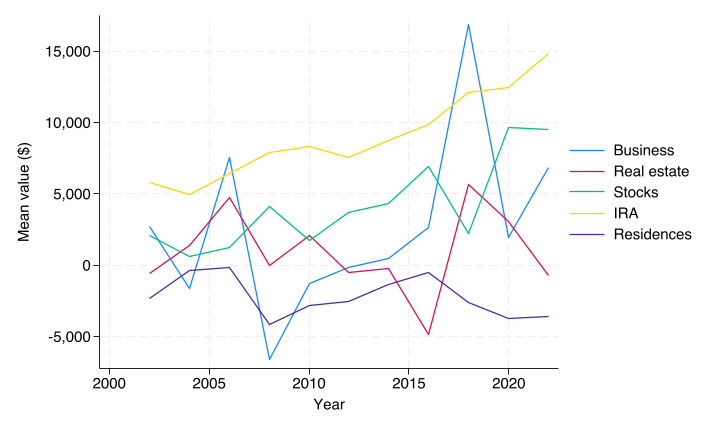
\includegraphics[width=0.8\textwidth]{../../Code/Descriptive/Figures/flows_by_asset_mean_by_year.png}
\caption{Average net investment flows across respondents}
\label{fig:flows_by_asset_mean_by_year}
\end{figure}
\FloatBarrier

\subsubsection{Defining wealth for assets and portfolios}

\par The final component needed for the returns calculations is the wealth held by a respondent (in the previous period). This is measured as the total stock in the given asset classes (core, retirement, and residential), and summing among these creates the stock of wealth in the given portfolios (core and retirement assets, net wealth). For example, \texttt{Net value of primary residences} and \texttt{Net value of primary residences} from the previous period are summed together as a measure of \textbf{wealth held in residential assets at the beginning of the previous period}. Figure ~\ref{fig:wealth_mean_by_year_panels} shows the mean wealth within these narrowly defined asset classes for each year of the survey. 

\begin{figure}[H]
\centering
\begin{minipage}[t]{0.48\textwidth}
\centering
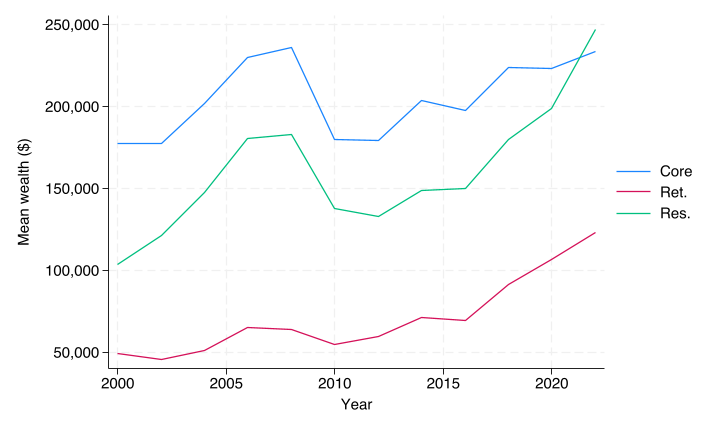
\includegraphics[width=\textwidth]{../../Code/Descriptive/Figures/wealth_mean_by_year_components.png}
\end{minipage}\hfill
\begin{minipage}[t]{0.48\textwidth}
\centering
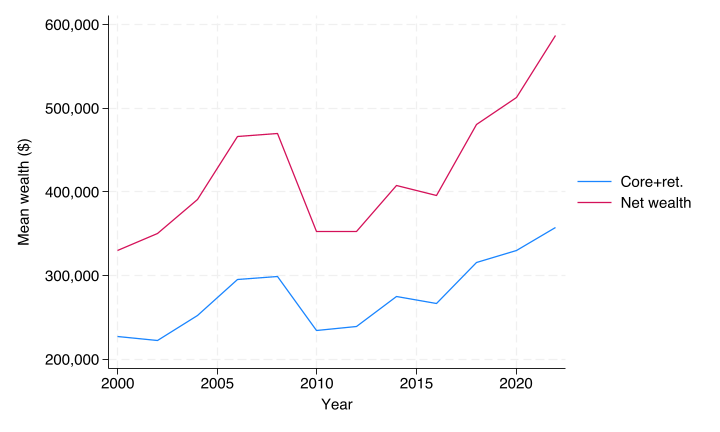
\includegraphics[width=\textwidth]{../../Code/Descriptive/Figures/wealth_mean_by_year_agg.png}
\end{minipage}
\caption{Mean wealth in asset classes and portfolios}
\label{fig:wealth_mean_by_year_panels}
\end{figure}
\FloatBarrier

\par Retirement assets seem to perform the worst in terms of average holdings. This may not be surprising, as the survey over samples older households and these households draw down their assets for consumption during retirement, in general. Core assets seem to offer the best performance, and all asset classes see a downward dive leading up to 2010 -- historically accurate in the context of investment performance during the global financial crisis.

 \par The following formula from \cite{Daminato2024} serves as a useful baseline for the return measures defined using HRS data: $$ r_t = \frac{y^c_t + cg_t -F_t -y^d_t}{A_{t-1} + .5F_t}   $$ where $y^c_t$ interest income and dividends, capital gains $cg_t$ measured as the difference between the reported stocks across waves of the survey\footnote{The capital gains to respondent $i$ for an asset $j$ is $V_{i,j,t} - V_{i,j,t-1}$, where $V_{i,j,t}$ is the value of the j-th asset for the i-th respondent in the t-th wave of the survey.}, $F_t$ net investment flows, $y^d_t$ payments on debt (in the RAND Longitudinal file, the variables mentioned are all in net terms, so this variable is equal to $0$), and $A_{t-1}$ total net wealth at the beginning of the previous period.
%%%%%%%%%%

\par Although this return measure is useful, the RAND HRS Longitudinal product has a unique structure that will guide how I define the asset classes and portfolios for which returns are accrued. As mentioned before, core assets are the most narrowly defined asset class here because interest income and dividends do not disaggregate into the asset classes: stocks, bonds, private business, IRA/Keogh.

 \subsubsection{Narrow asset classes}
 
\par Recall that we define the interest income and dividends to core assets as the RAND variable for \texttt{Household Capital Income} (\texttt{HwICAP}), which sums together the interest income and dividends to the following underlying assets of interest: stocks, bonds, business, and real estate. Since interest income is an important component of the return calculation, we define the returns to core assets in the following way. I find the variables capital gains and net investment flows to each of these assets and aggregate them to reach a measure of capital gains on core assets and net investment flows to core assets.  

\par The returns to the core assets are given by

$$ r^{core}_{it} = \frac{y^{core}_{it} + cg^{core}_{it} - F^{core}_{it}}{A^{core}_{i,t-1} + .5F^{core}_{it}}   $$

where $y^{core}_{it}$ is the interest income and dividends on the core assets, $cg^{core}_{it}$ are the capital gains on the core assets, $F^{core}_{it}$ are the net investment flows to core assets, and importantly, $A^{core}_{i,t-1}$ is the total wealth held in core assets in the previous period.

\par The rest of the return measures are defined similarly. In the HRS data, we also observe income on retirement assets. This allows us to define a return measure for retirement assets

$$ r^{ret}_{it} = \frac{y^{ret}_{it} + cg^{ret}_{it} - F^{ret}_{it}}{A^{ret}_{i,t-1} + .5F^{ret}_{it}}   $$

where $y^{ret}_{it}$ is the interest income and dividends on the retirement assets, $cg^{ret}_{it}$ are the capital gains on retirement assets, $F^{ret}_{it}$ are the net investment flows to retirement assets, and $A^{ret}_{i,t-1}$ is the total wealth held in retirement assets in the previous period.

\par Based on the modules offered in a given survey wave, I assume that there are no interest income or dividends to primary and secondary residential assets, so that the interest income and dividends accrued to residential assets are 0 in a given period $(y^{res}_{it}=0)$. Thus, I define returns to residential assets as

$$ r^{res}_{it} = \frac{cg^{res}_{it} - F^{res}_{it}}{A^{res}_{i,t-1} + .5F^{res}_{it}}   $$

where  $cg^{res}_{i,t}$ are the capital gains on the residential assets, $F^{res}_{i,t}$ are the net investment flows to residential assets (including improvement costs), and $A^{res}_{i,t-1}$ is the total value of the residential assets in the previous period.

\subsubsection{Broad asset classes}

\par After defining the returns for narrow asset classes, I also define the return measure for portfolios (returns on multiple assets). The first portfolio definition is for returns to core and retirement assets: 

$$ r^{coret}_{it} = \frac{y^{coret}_{it} + cg^{coret}_{it} - F^{coret}_{it}}{A^{coret}_{i,t-1} + .5F^{coret}_{it}}   $$

where $y^{coret}_{it}$ is the interest income and dividends on core and retirement assets, $cg^{coret}_{it}$ are the capital gains on core and retirement assets, $F^{coret}_{it}$ are the net investment flows to core and retirement assets, and $A^{coret}_{i,t-1}$ is the total wealth held in core and retirement assets in the previous period.

\par The broadest portfolio definition is for total net wealth holdings. Returns to net wealth are given by

$$ r^{net}_{it} = \frac{y^{net}_{it} + cg^{net}_{it} - F^{net}_{it}}{A^{net}_{i,t-1} + .5F^{net}_{it}}   $$

where $y^{net}_{it}$ is the interest income and dividends on core and retirement assets, $cg^{net}_{it}$ are the capital gains on all available asset classes in the survey, $F^{net}_{it}$ are the net investment flows on assets for which it is relevant in the survey (stocks, bonds, business, IRA, residences, and real estate), and $A^{net}_{i,t-1}$ is the total value of the available assets minus liabilities in the previous period\footnote{\texttt{Value of all mortgages/land contracts (secondary residence)} (\texttt{HwAMRTB}) is an optional question in some survey waves so it is omitted from the list of liabilities used to compute net wealth.}.

\subsubsection{The distribution of measured returns}

\par I present the the evolution of the return measures, averaged over the respondents, over time in the following figure ~\ref{fig:returns_mean_by_year_panels}. I group them by asset classes (core, retirement, residential) and portfolio definitions (core and retirement, net wealth). %%%%describe%%%%%%

\begin{figure}[H]
\centering
\begin{minipage}[t]{0.48\textwidth}
\centering
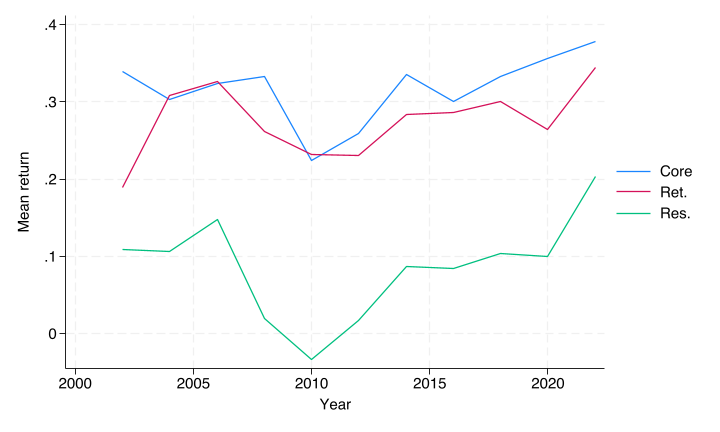
\includegraphics[width=\textwidth]{../../Code/Descriptive/Figures/returns_mean_by_year_components.png}
\end{minipage}\hfill
\begin{minipage}[t]{0.48\textwidth}
\centering
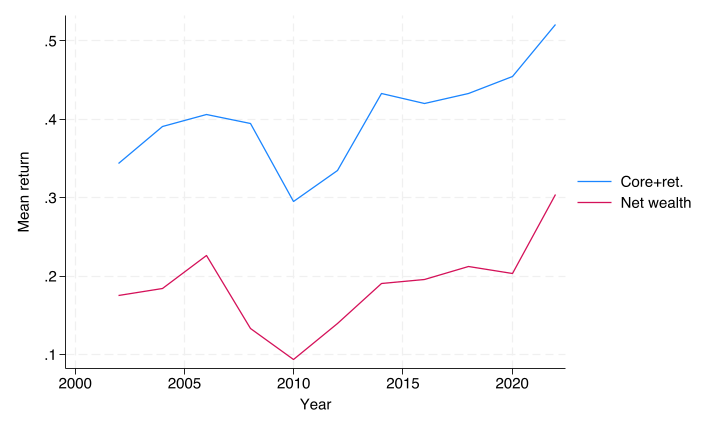
\includegraphics[width=\textwidth]{../../Code/Descriptive/Figures/returns_mean_by_year_agg.png}
\end{minipage}
\caption{Mean returns for asset classes and portfolios}
\label{fig:returns_mean_by_year_panels}
\end{figure}
\FloatBarrier

\par Mean returns to core assets seem to have the best performance in terms of asset classes, followed by retirement and then residential assets. For portfolios, returns to net wealth are lower than returns to core and retirement assets on average. Across asset classes (and thus portfolios), there is a decline in returns on average in 2010, which is likely an artifact of the economic downturn associated with the Global Financial Crisis of 2008.

\par Figure~\ref{fig:returns_histogram_components_pooled} shows the distribution of returns across person-years, pooled over survey waves (2002--2022), for the three asset classes: core, retirement, and residential. 

\begin{figure}[H]
\centering
\begin{minipage}[t]{0.48\textwidth}
\centering
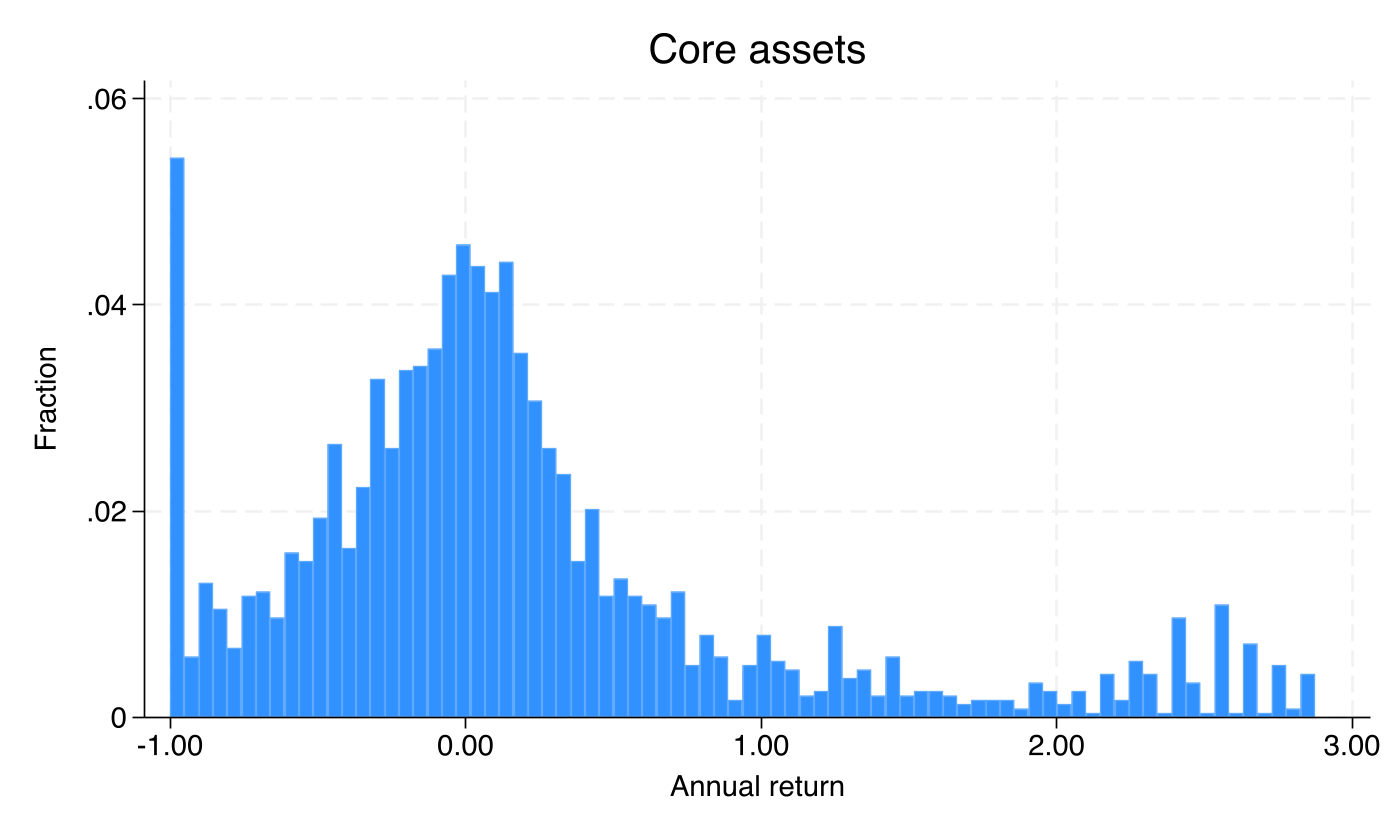
\includegraphics[width=\textwidth]{../../Code/Descriptive/Figures/returns_hist_r1_pooled.png}
\end{minipage}\hfill
\begin{minipage}[t]{0.48\textwidth}
\centering
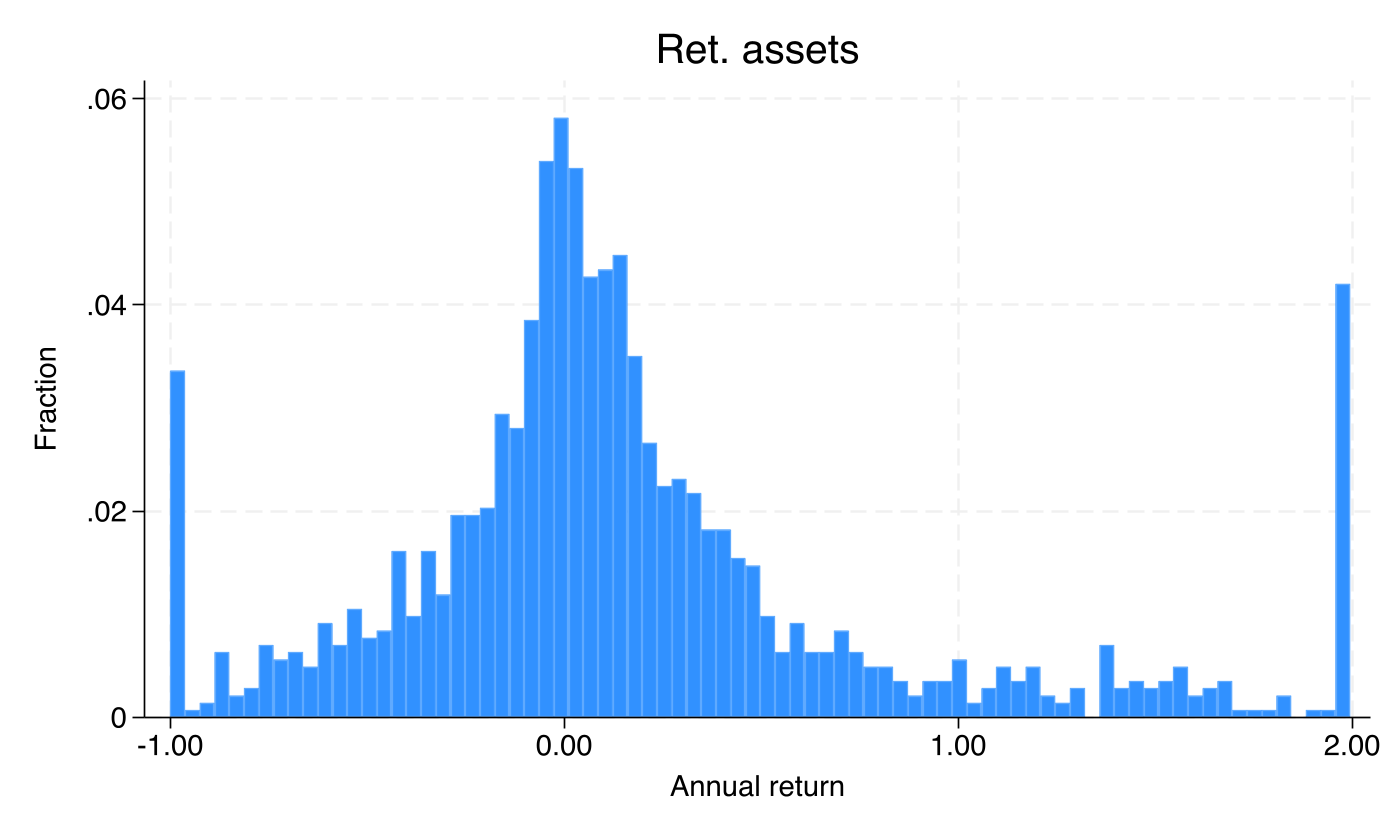
\includegraphics[width=\textwidth]{../../Code/Descriptive/Figures/returns_hist_r2_pooled.png}
\end{minipage}

\vspace{0.5em}

\begin{minipage}[t]{0.48\textwidth}
\centering
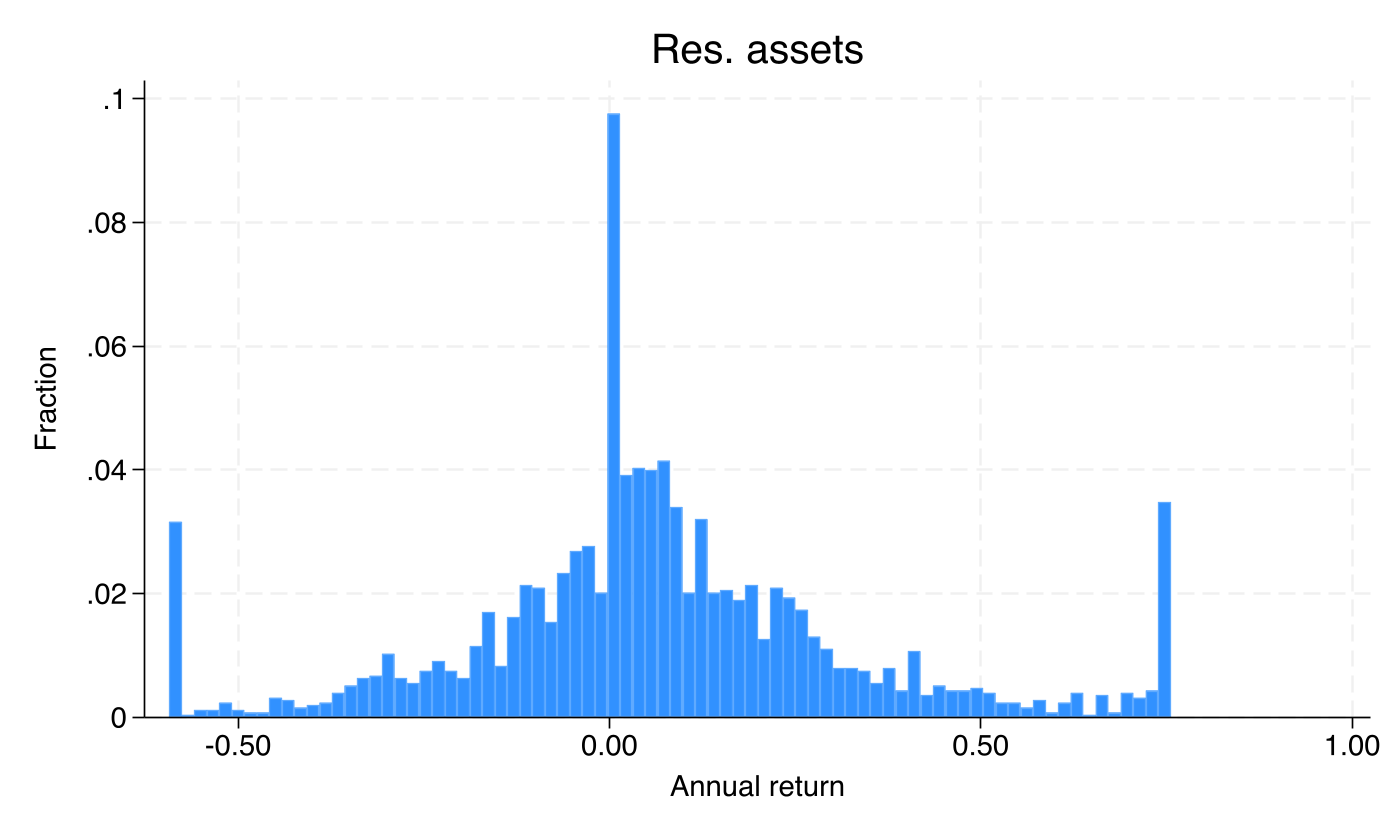
\includegraphics[width=\textwidth]{../../Code/Descriptive/Figures/returns_hist_r3_pooled.png}
\end{minipage}
\caption{Histogram for distribution of returns to the defined asset classes}
\label{fig:returns_histogram_components_pooled}
\end{figure}
\FloatBarrier

\par In particular, the distribution of returns to core assets has a right tail with extremely high values relative to the distribution of returns to retirement and residential assets. Each distribution seems to be centered near $0$, which is a good sign. Residential assets feature a significant share of respondents earning a positive return; this is in line with the empirical fact that home ownership in the United States is relatively common compared to investment in other asset classes. 

\par Figure~\ref{fig:returns_histogram_agg_pooled} shows the distribution of returns for the constructed portfolio measures: core and retirement assets and net wealth. In general, these figures are encouraging, as its shape closely resembles other estimates of the empirical distribution of individual realized returns using other datasets. 

\begin{figure}[H]
\centering
\begin{minipage}[t]{0.48\textwidth}
\centering
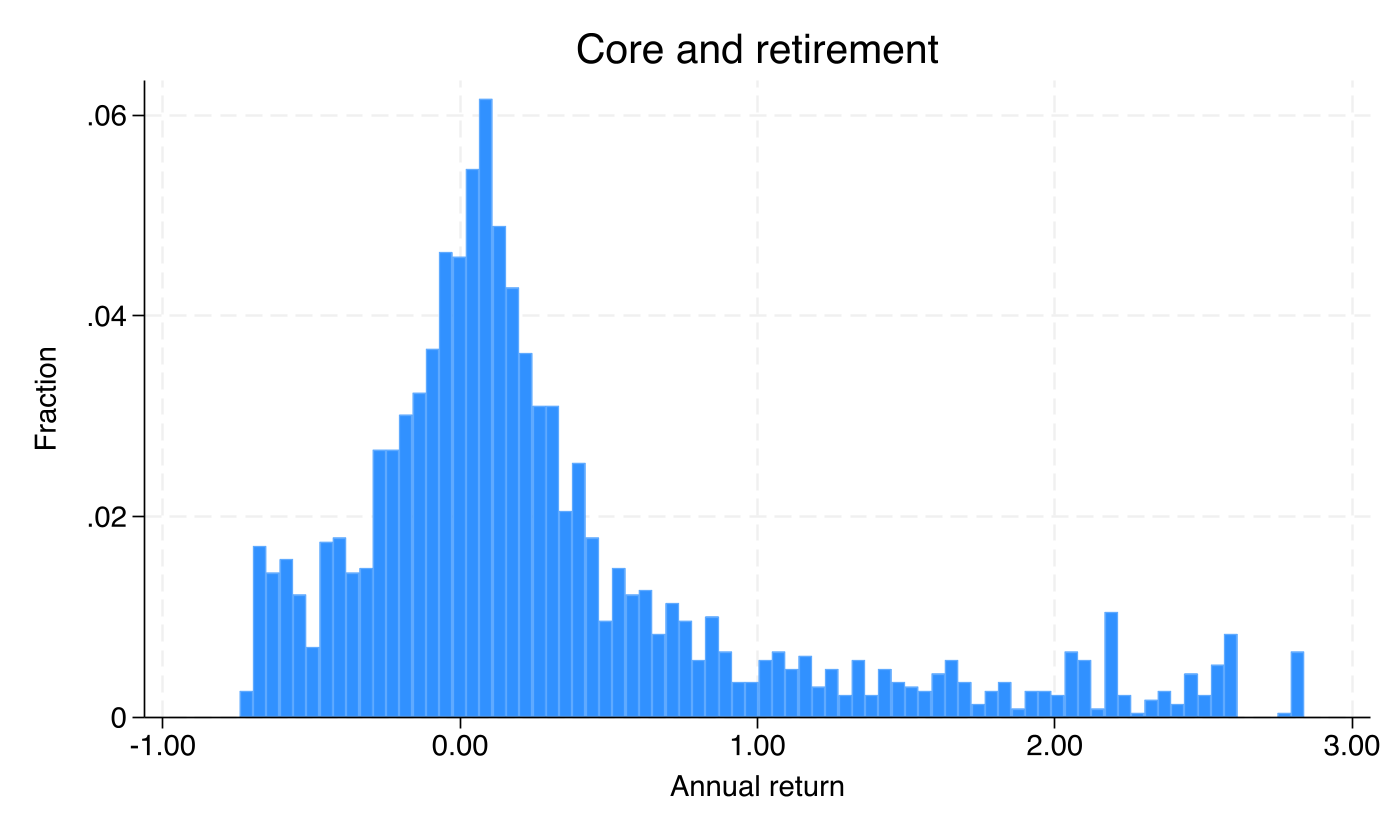
\includegraphics[width=\textwidth]{../../Code/Descriptive/Figures/returns_hist_r4_pooled.png}
\end{minipage}\hfill
\begin{minipage}[t]{0.48\textwidth}
\centering
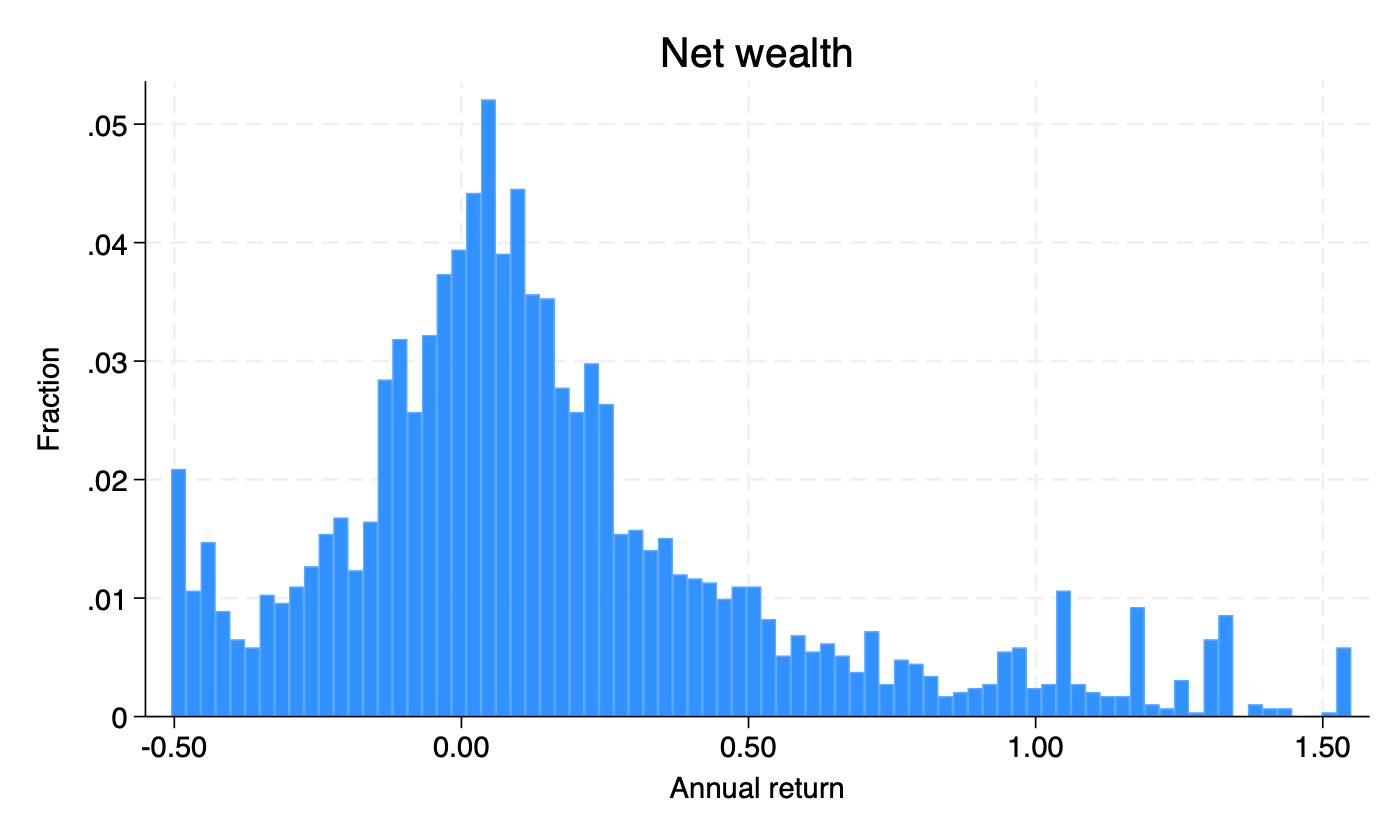
\includegraphics[width=\textwidth]{../../Code/Descriptive/Figures/returns_hist_r5_pooled.png}
\end{minipage}
\caption{Histogram for distribution of returns to the defined portfolios}
\label{fig:returns_histogram_agg_pooled}
\end{figure}
\FloatBarrier

\par Table~\ref{tab:returns_portfolio_moments_pooled} summarizes the distribution of returns (mean, standard deviation, skewness, kurtosis and selected percentiles) for each asset class and portfolio, pooling person-years in the same sample as Figure~\ref{fig:returns_histogram_components_pooled} and the return-by-age and return-by-education tables (pooled OLS sample for $r^{net}$ on generalized trust with education categories and standard panel controls). A major takeaway from this table is that \textit{the mean returns across both asset classes and portfolios are much higher than the median}. This suggests that there are a significant number of respondents with computed returns that are extremely large.

\begin{table}[htbp]\centering\small
\caption{Returns to assets/portfolios}
\label{tab:returns_portfolio_moments_pooled}
\begin{tabular}{lrrrrrrr}\toprule
Returns to & Mean & SD & Skewness & Kurtosis & P1 & P50 & P99 \\\\ \midrule
Core assets & 0.3066 & 1.5804 & 7.45 & 97.65 & -1.0000 & 0.0249 & 6.6292 \\\\
Residential assets & 0.0777 & 0.3935 & 3.38 & 41.27 & -1.0000 & 0.0422 & 1.3805 \\\\
Retirement assets & 0.2666 & 1.1189 & 5.90 & 62.82 & -1.0000 & 0.0575 & 5.3233 \\\\
\addlinespace
Core and retirement assets & 0.3905 & 1.2199 & 7.41 & 107.65 & -0.9413 & 0.1138 & 4.9135 \\\\
Net wealth & 0.2011 & 0.6305 & 4.48 & 38.68 & -0.7085 & 0.0843 & 2.6968 \\\\
\bottomrule
\end{tabular}
\end{table}

\FloatBarrier

\subsection{Demographic variables}

\par The HRS offers a collection of trust questions in \say{Section V: Modules} section of the 2020 survey. There are a total of 8 questions, and the one I focus on in this paper is \texttt{Trust: People in General} (\texttt{RV557}):

\begin{itemize}
  \item ``How much do you trust people in general?''
  \end{itemize}

Respondents are asked to give an answer between 1 and 10. This set of trust questions was only a part of the questionnaire in that year. This is an issue, since the panel structure of the HRS allows me to estimate the persistent component of returns, variation in the trust measure would be ideal if it matters for trust. That said, in the panel setting, we can assume that trust, like education, is fixed over time.\footnote{Literature on trust talks about how history of being cheated or treated fairly form individuals' trust over time. If this is true and at some point, one learns enough and forms their trust level, then a sample with an over-representation of older household is a reasonable environment to assume constant trust levels.}

\par Figure~\ref{fig:39_trust_general_2020_hist} shows the distribution of responses to the trust question. Interestingly, most of the respondents report a trust level of 5 or 7. In addition, there are a significant number of respondents who report trusting other people at the most extreme values (0 or 10). This suggests that the sample has a significant number of individuals who are very trusting and also very distrusting. In general, 

\begin{figure}[H]
\centering
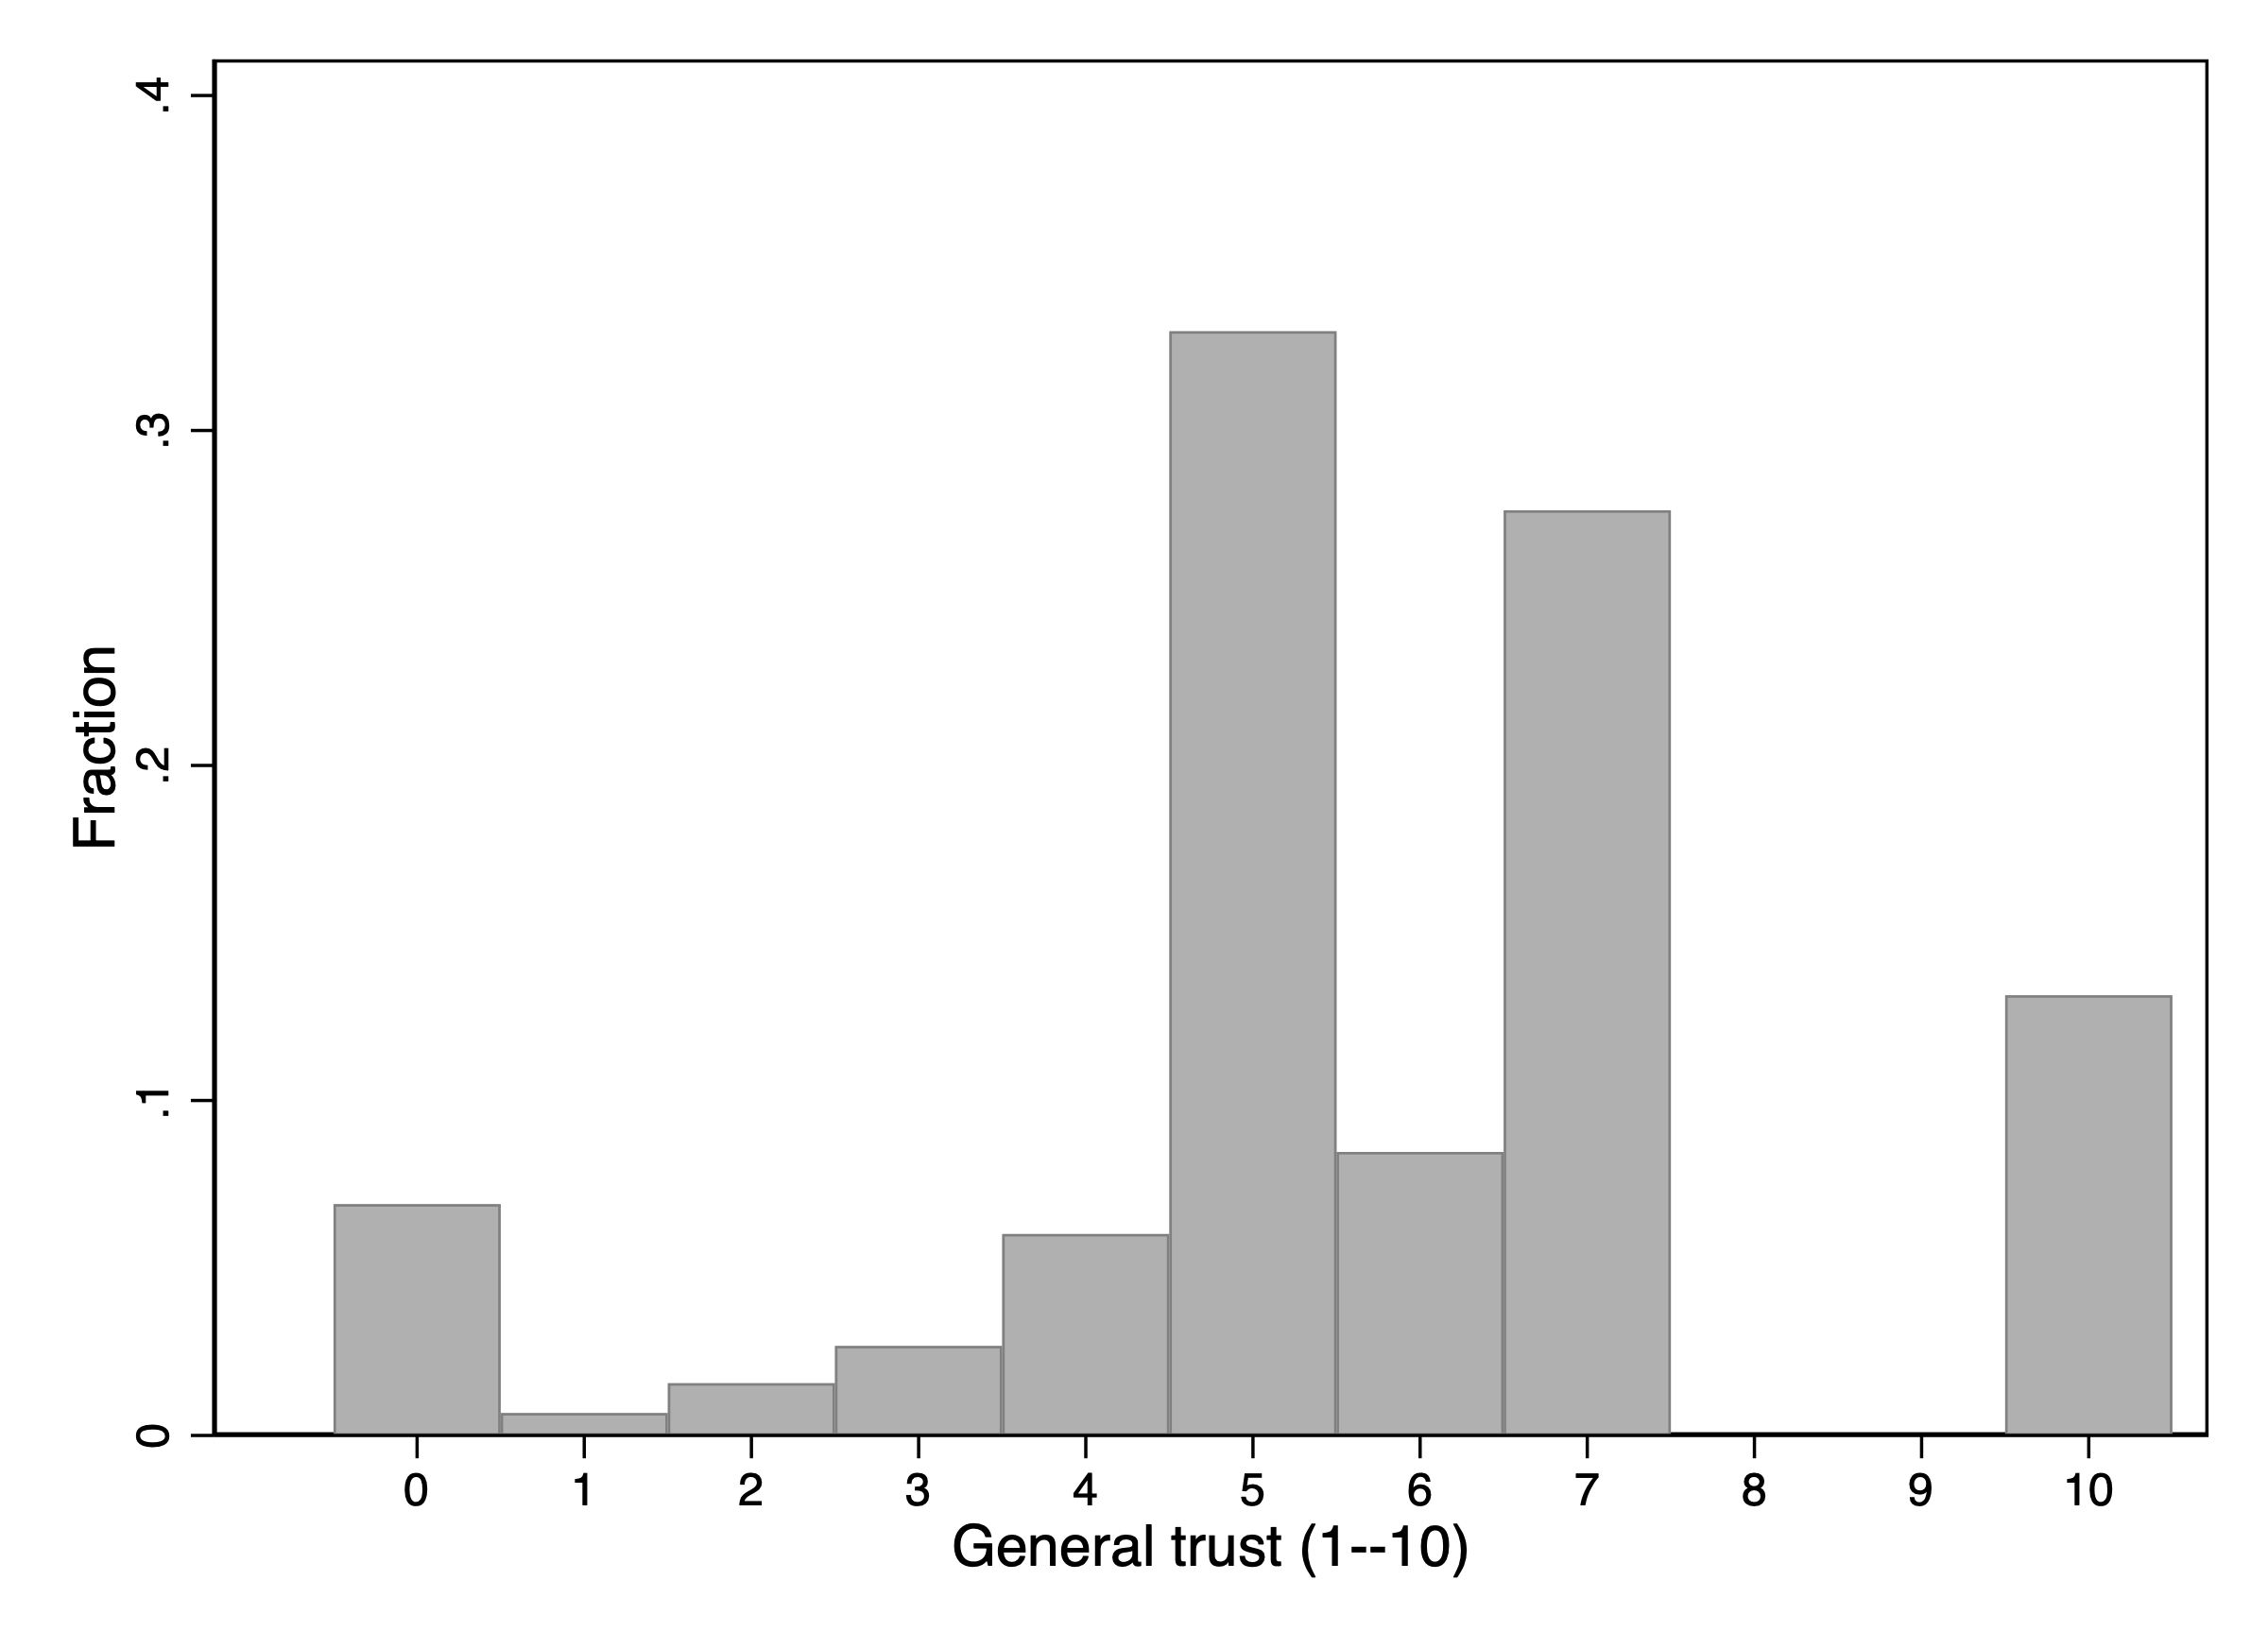
\includegraphics[width=0.72\textwidth]{../../Code/Descriptive/Figures/39_trust_general_2020_hist.png}
\caption{Distribution of responses to the \texttt{Trust} survey question}
\label{fig:39_trust_general_2020_hist}
\end{figure}
\FloatBarrier

\par Figure~\ref{fig:trust_mean_by_race_eth_2020} summarizes the average trust responses by race and ethnicity. As can be seen in Appendix Table~\ref{tab:42_trust_determinants} (\textit{Determinants of General Trust}), the race variable (in particular, the \texttt{Black} racial group) is robustly found to be predictive of and negatively correlated with trust. Minority groups, especially \texttt{Black}, report lower trust levels on average than their white counterparts in the sample. 

\begin{figure}[H]
\centering
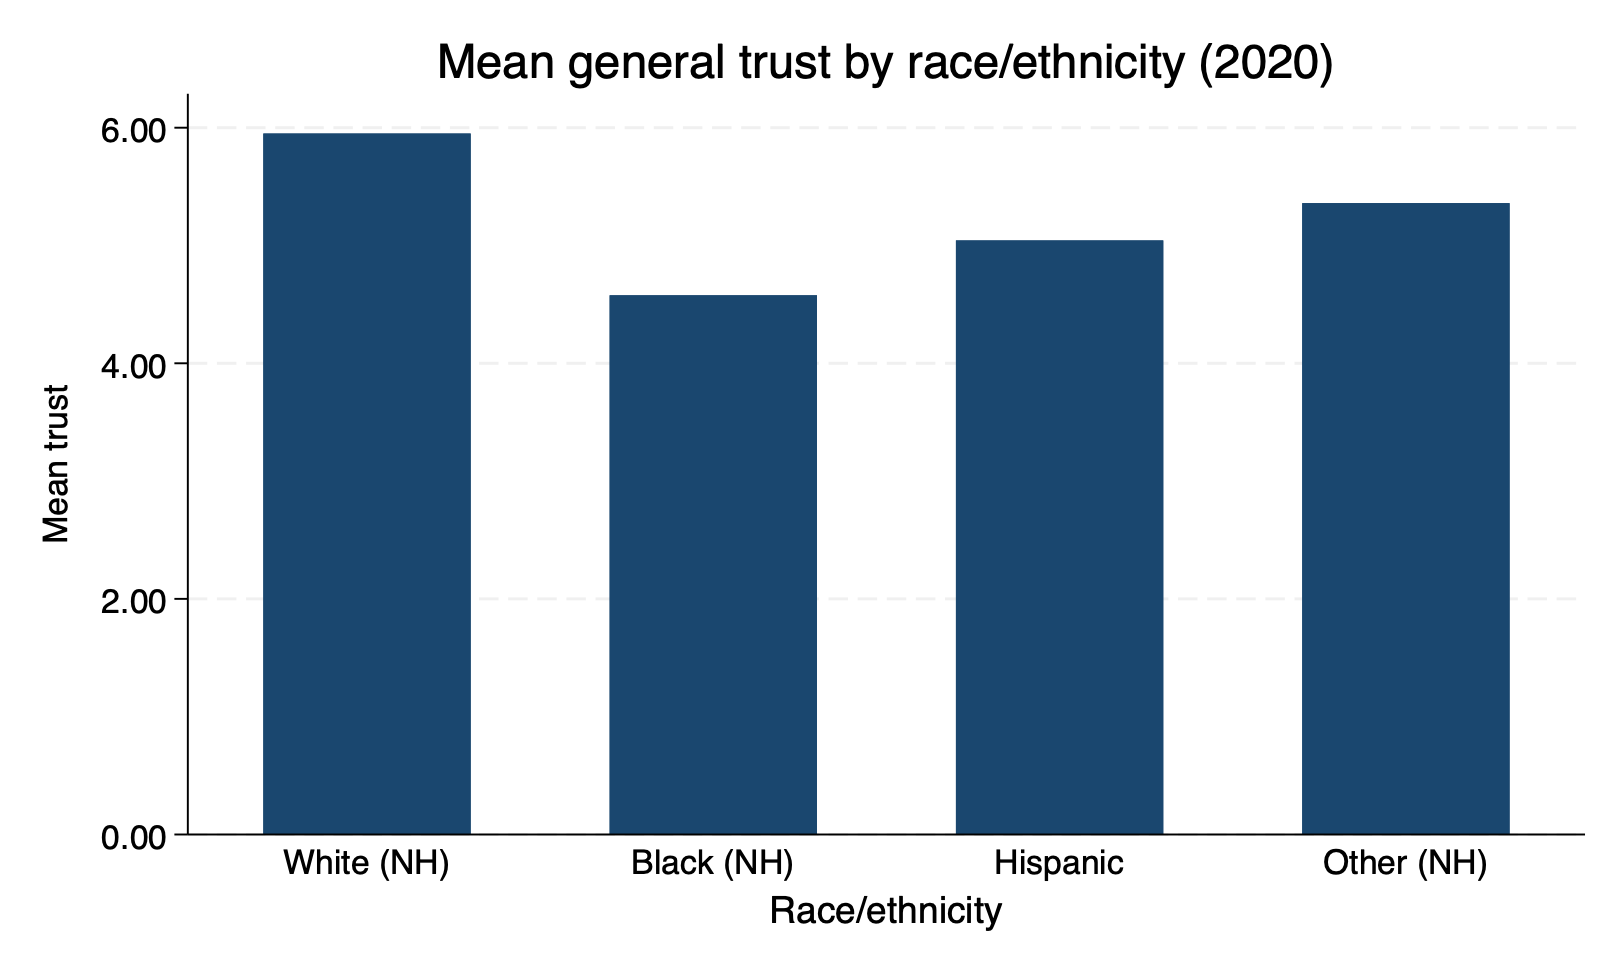
\includegraphics[width=0.72\textwidth]{../../Code/Descriptive/Figures/trust_mean_by_race_eth_2020.png}
\caption{Average \texttt{Trust} responses conditional on \texttt{Race}}
\label{fig:trust_mean_by_race_eth_2020}
\end{figure}
\FloatBarrier

% Tighter layout for wide tables (same macro as results.tex/extensions.tex/appendix.tex).
\providecommand{\ChapterTableNoteText}[1]{\parbox[t]{0.94\textwidth}{#1}}
\providecommand{\InputStataRegTableCompact}[4]{%
\begin{table}[htbp]
\centering
\caption{#1}%
\label{#2}%
\begin{threeparttable}
\begingroup
\footnotesize
\setlength{\tabcolsep}{4pt}%
\renewcommand{\arraystretch}{0.94}%
\resizebox{\textwidth}{!}{%
\input{#3}%
}%
\endgroup
\begin{tablenotes}[flushleft]
\footnotesize
\item \ChapterTableNoteText{#4}%
\end{tablenotes}
\end{threeparttable}
\end{table}%
}

\par Table~\ref{tab:39_reg_sample_demographics} summarizes the relevant baseline control variables (\texttt{Years of Schooling} (\texttt{RAEDYRS}) and \texttt{Labor Force Status} (\texttt{RwLBRF})) and the extended set of control vairables(\texttt{Gender} (\texttt{RAGENDER}), \texttt{Race} (\texttt{RARACEM}), \texttt{Whether Hispanic} (\texttt{RAHISPAN})\footnote{The two \texttt{Race, Ethnicity} variables are combined to create the racial categories: NH White, NH Black, Hispanic, NH Other.}, \texttt{Place of Birth} (\texttt{RABPLACE}), and \texttt{Census Region} (\texttt{RwCENREG})) relevant for the regression models. Notice that the summary statistic (proportion of respondents for the categorical variables) 2020 demographic variables seem to be very close to the pooled versions of those same variables. This is a good sign, since trust is only measured in 2020.

\par The data suggests that more than half of the sample has at least some college, and less than a third of the respondents are working full-time. Most respondents are married and were born in the United States. In terms of geographic location, respondents seem to be concentrated in the South census region. 

\begin{table}[H]
\centering
\caption{\textbf{Sample Demographics}}
\label{tab:39_reg_sample_demographics}
\begin{threeparttable}
\begingroup
\setlength{\tabcolsep}{4pt}%
\renewcommand{\arraystretch}{0.94}%
\resizebox{\textwidth}{!}{%
\begin{tabular*}{\linewidth}{@{\extracolsep{\fill}}lrr}\toprule
 & \multicolumn{1}{c}{(1)} & \multicolumn{1}{c}{(2)} \\
\midrule
\multicolumn{3}{@{}l}{\textit{Panel A: Education categories and labor force}} \\
\midrule
Share: Less HS &  0.183 &  0.192 \\
Share: HS Grad &  0.258 &  0.291 \\
Share: Some College &  0.247 &  0.242 \\
Share: College &  0.158 &  0.135 \\
Share: Postgrad &  0.154 &  0.141 \\
Share in labor force &  0.305 &  0.373 \\
\addlinespace
\multicolumn{3}{@{}l}{\textit{Panel B: Gender, marital status, race/ethnicity, birthplace, and census region}} \\
\midrule
Share female &  0.537 &  0.554 \\
Share married &  0.630 &  0.681 \\
Share: NH White &  0.612 &  0.680 \\
Share: NH Black &  0.198 &  0.163 \\
Share: Hispanic &  0.149 &  0.121 \\
Share: NH Other &  0.038 &  0.035 \\
Share born in U.S. &  0.833 &  0.877 \\
Share: Northeast &  0.147 &  0.129 \\
Share: Midwest &  0.198 &  0.231 \\
Share: South &  0.448 &  0.451 \\
Share: West &  0.205 &  0.182 \\
\bottomrule\end{tabular*}
%
}%
\endgroup
\begin{tablenotes}[flushleft]
\footnotesize
\item \ChapterTableNoteText{Column~(1) reports shares for the 2020 cross-section; column~(2) reports shares pooled across all survey years.}%
\end{tablenotes}
\end{threeparttable}
\end{table}


\subsection{Descriptive statistics for returns to net wealth}

 
\par Since regression analysis focuses on returns to net wealth, this section will offer a number of decompositions of returns to net wealth by wealth, age, employment, and education. 

\subsubsection{Return vs.\ net wealth}

\par Figure~\ref{fig:39_r5_netwealth_pct} is the appropriate place to read the raw relationship between returns and wealth in the sample. For returns to net wealth, that descriptive relationship appears fairly weak and close to flat, with at most a slight positive tilt in the fitted line. That said the observations towards the ends of the net wealth distribution do seem to exhibit the \textit{scale dependence} result found in the literature regarding returns.

\begin{figure}[H]
\centering
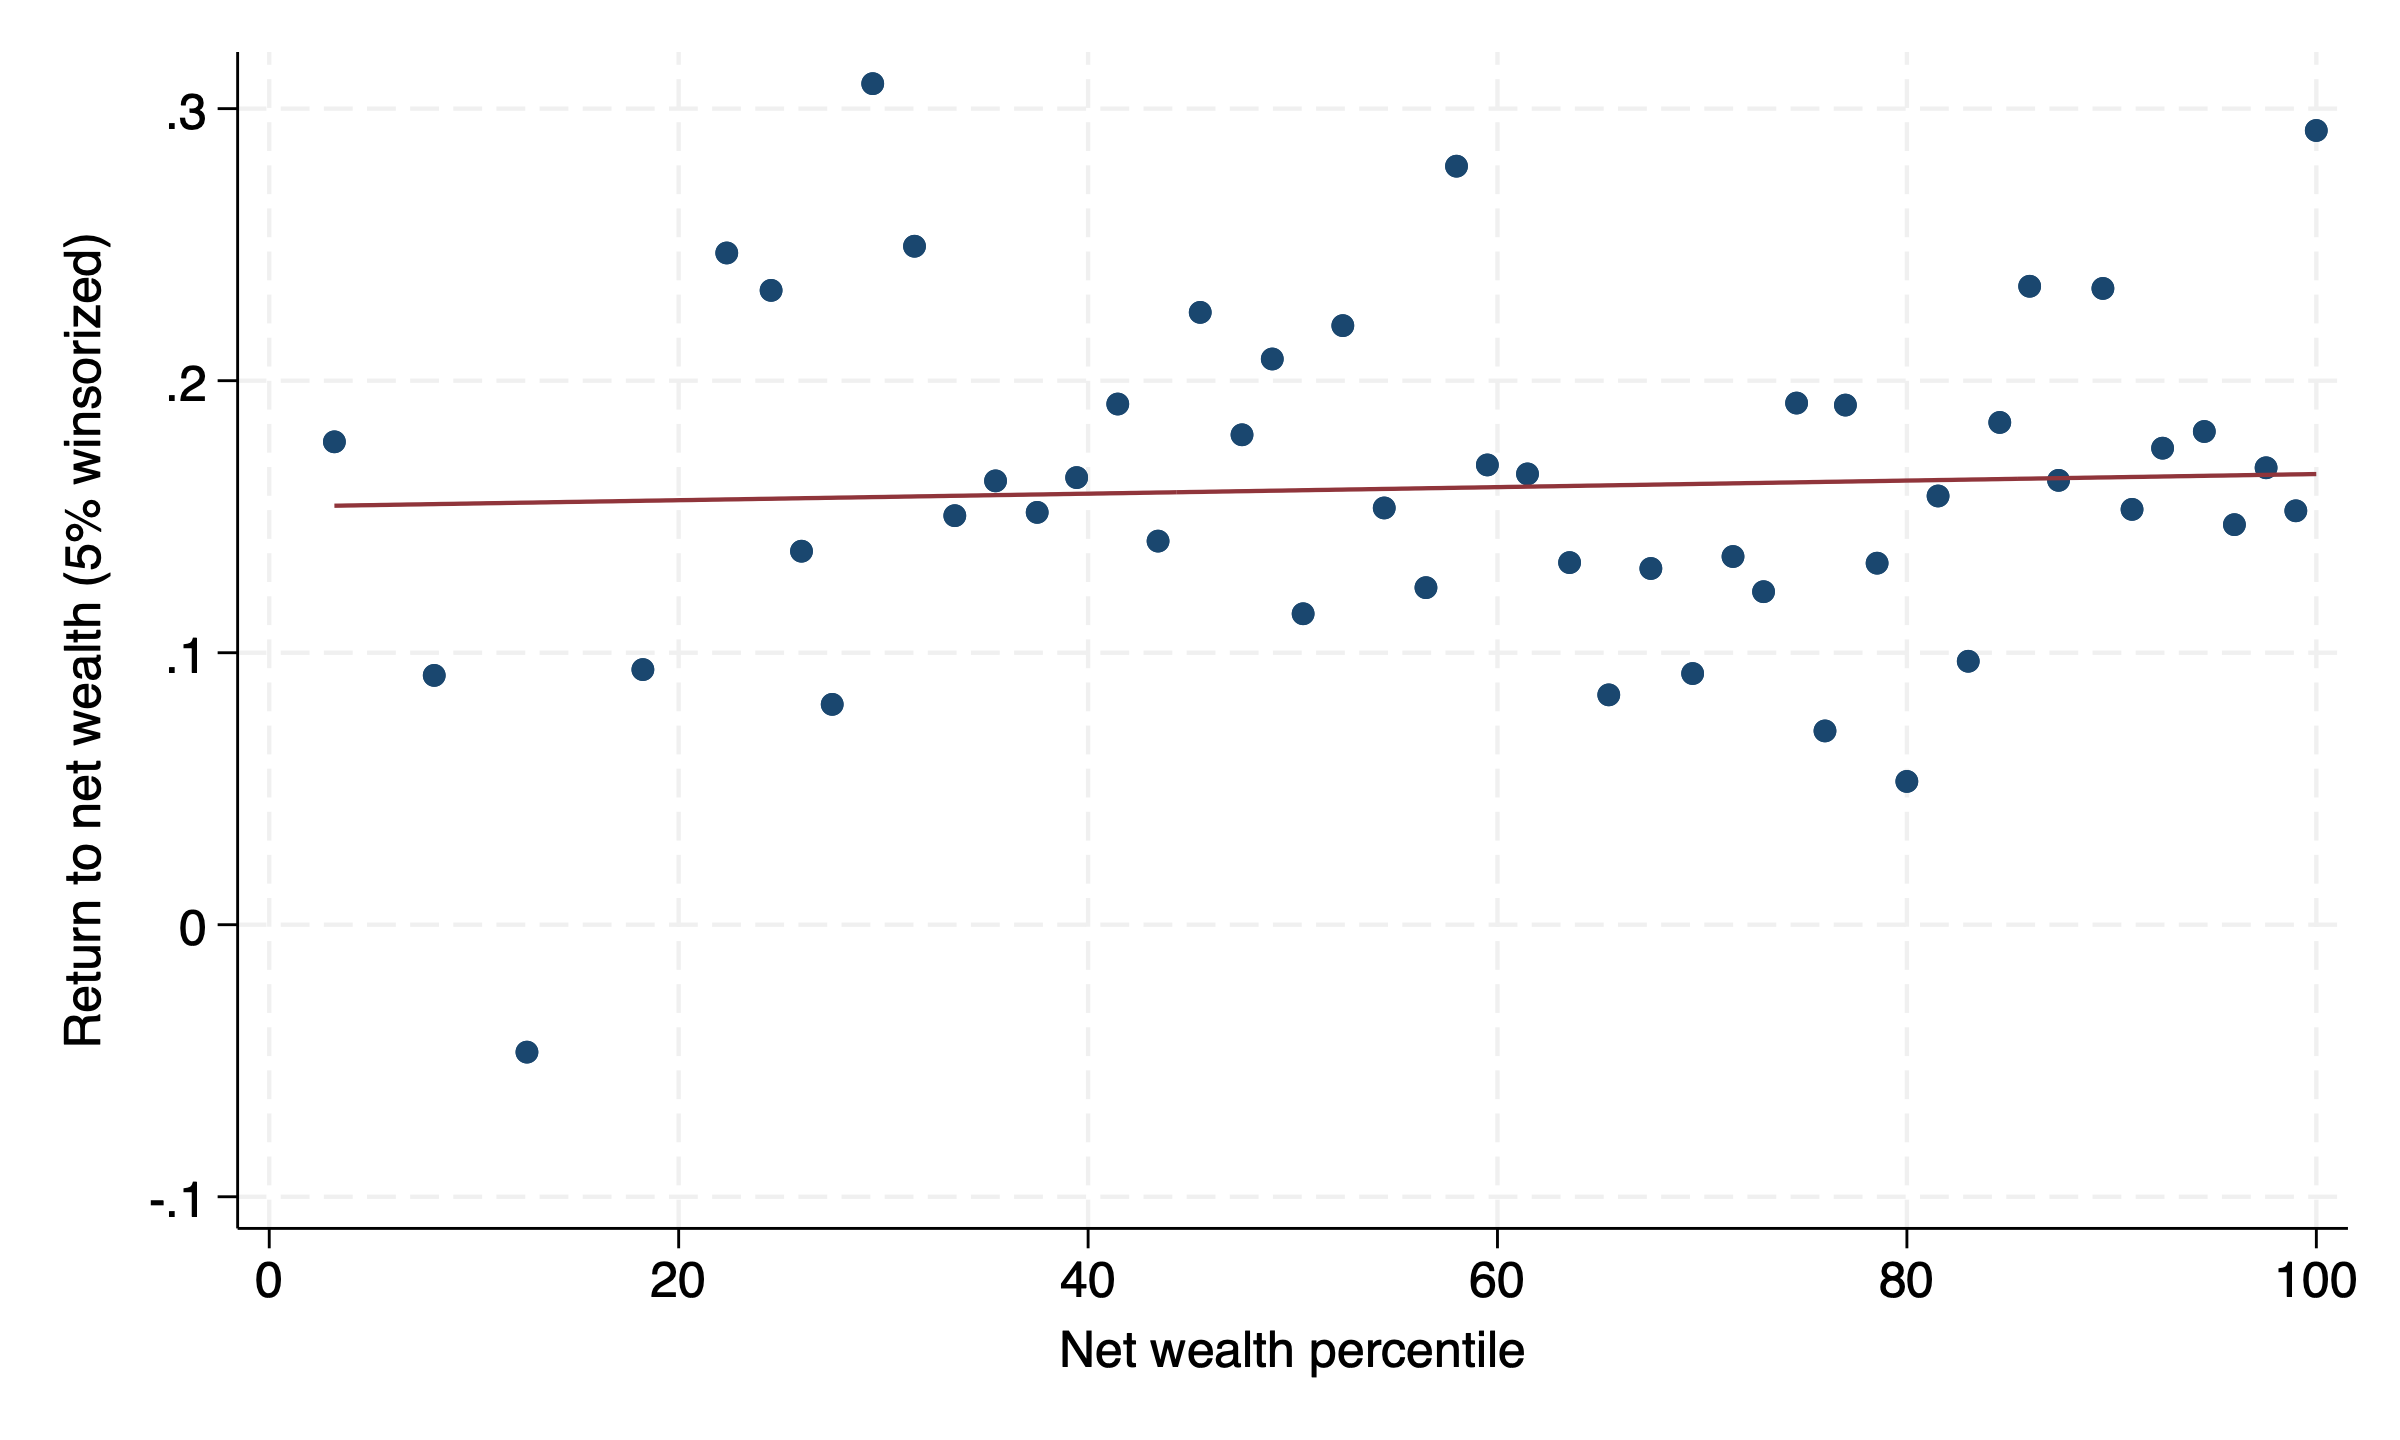
\includegraphics[width=0.8\textwidth]{../../Code/Descriptive/Figures/39_pooled_r5_vs_netwealth_pct.png}
\caption{Returns to net wealth vs.\ net wealth percentile}
\label{fig:39_r5_netwealth_pct}
\end{figure}
\FloatBarrier

\subsubsection{Returns by age and education}

\par \texttt{Age at Interview} (\texttt{RwAGEY\_B}) and \texttt{Years of Schooling} are control variables which are thought to matter empirically for both trust and returns. Since each of these play a unique role in the HRS data (education time-invariant, age is higher on average due to oversampling of retirees), a decomposition of returns by each of these should be considered. Table~\ref{tab:39_r5_age_bin} reports moments of the returns to net wealth distribution conditional on age. 

\InputStataRegTableCompact{\textbf{Return to Net Wealth by Age}}{tab:39_r5_age_bin}{../../Code/Descriptive/Tables/39_r5_by_age_bin.tex}{}
\FloatBarrier

\par A very interesting feature of the sample is that there are less than twenty respondents between the ages of 30 and 44, and less than 40 respondents between the ages of 30 and 49. The majority of the respondents are between the ages of 60 and 79.

\par Table~\ref{tab:39_r5_educ_cat} reports moments of the returns to net wealth distribution conditional on education. In general, it appears that more years of schooling lead to lower average returns to net wealth, but also less volatility as measured by the standard deviation. Interestingly, the group of respondents that did not complete high school have the highest returns on average in the sample. 

\InputStataRegTableCompact{\textbf{Return to Net Wealth by Education}}{tab:39_r5_educ_cat}{../../Code/Descriptive/Tables/39_r5_by_educ_cat.tex}{ Education categories are constructed from RAND HRS years of education: Less HS ($<12$), HS Grad ($=12$), Some College ($13$--$15$), College ($=16$), Postgrad ($>16$).}
\FloatBarrier

\subsubsection{Return vs.\ labor force participation status}

\par Figure ~\ref{fig:39_r5_lf_year} shows the mean returns to net wealth conditional on labor foce paritipation status. Following the global financial crisis of 2008, it seems that returns are higher on average conditional on being employed in general. 

\begin{figure}[H]
\centering
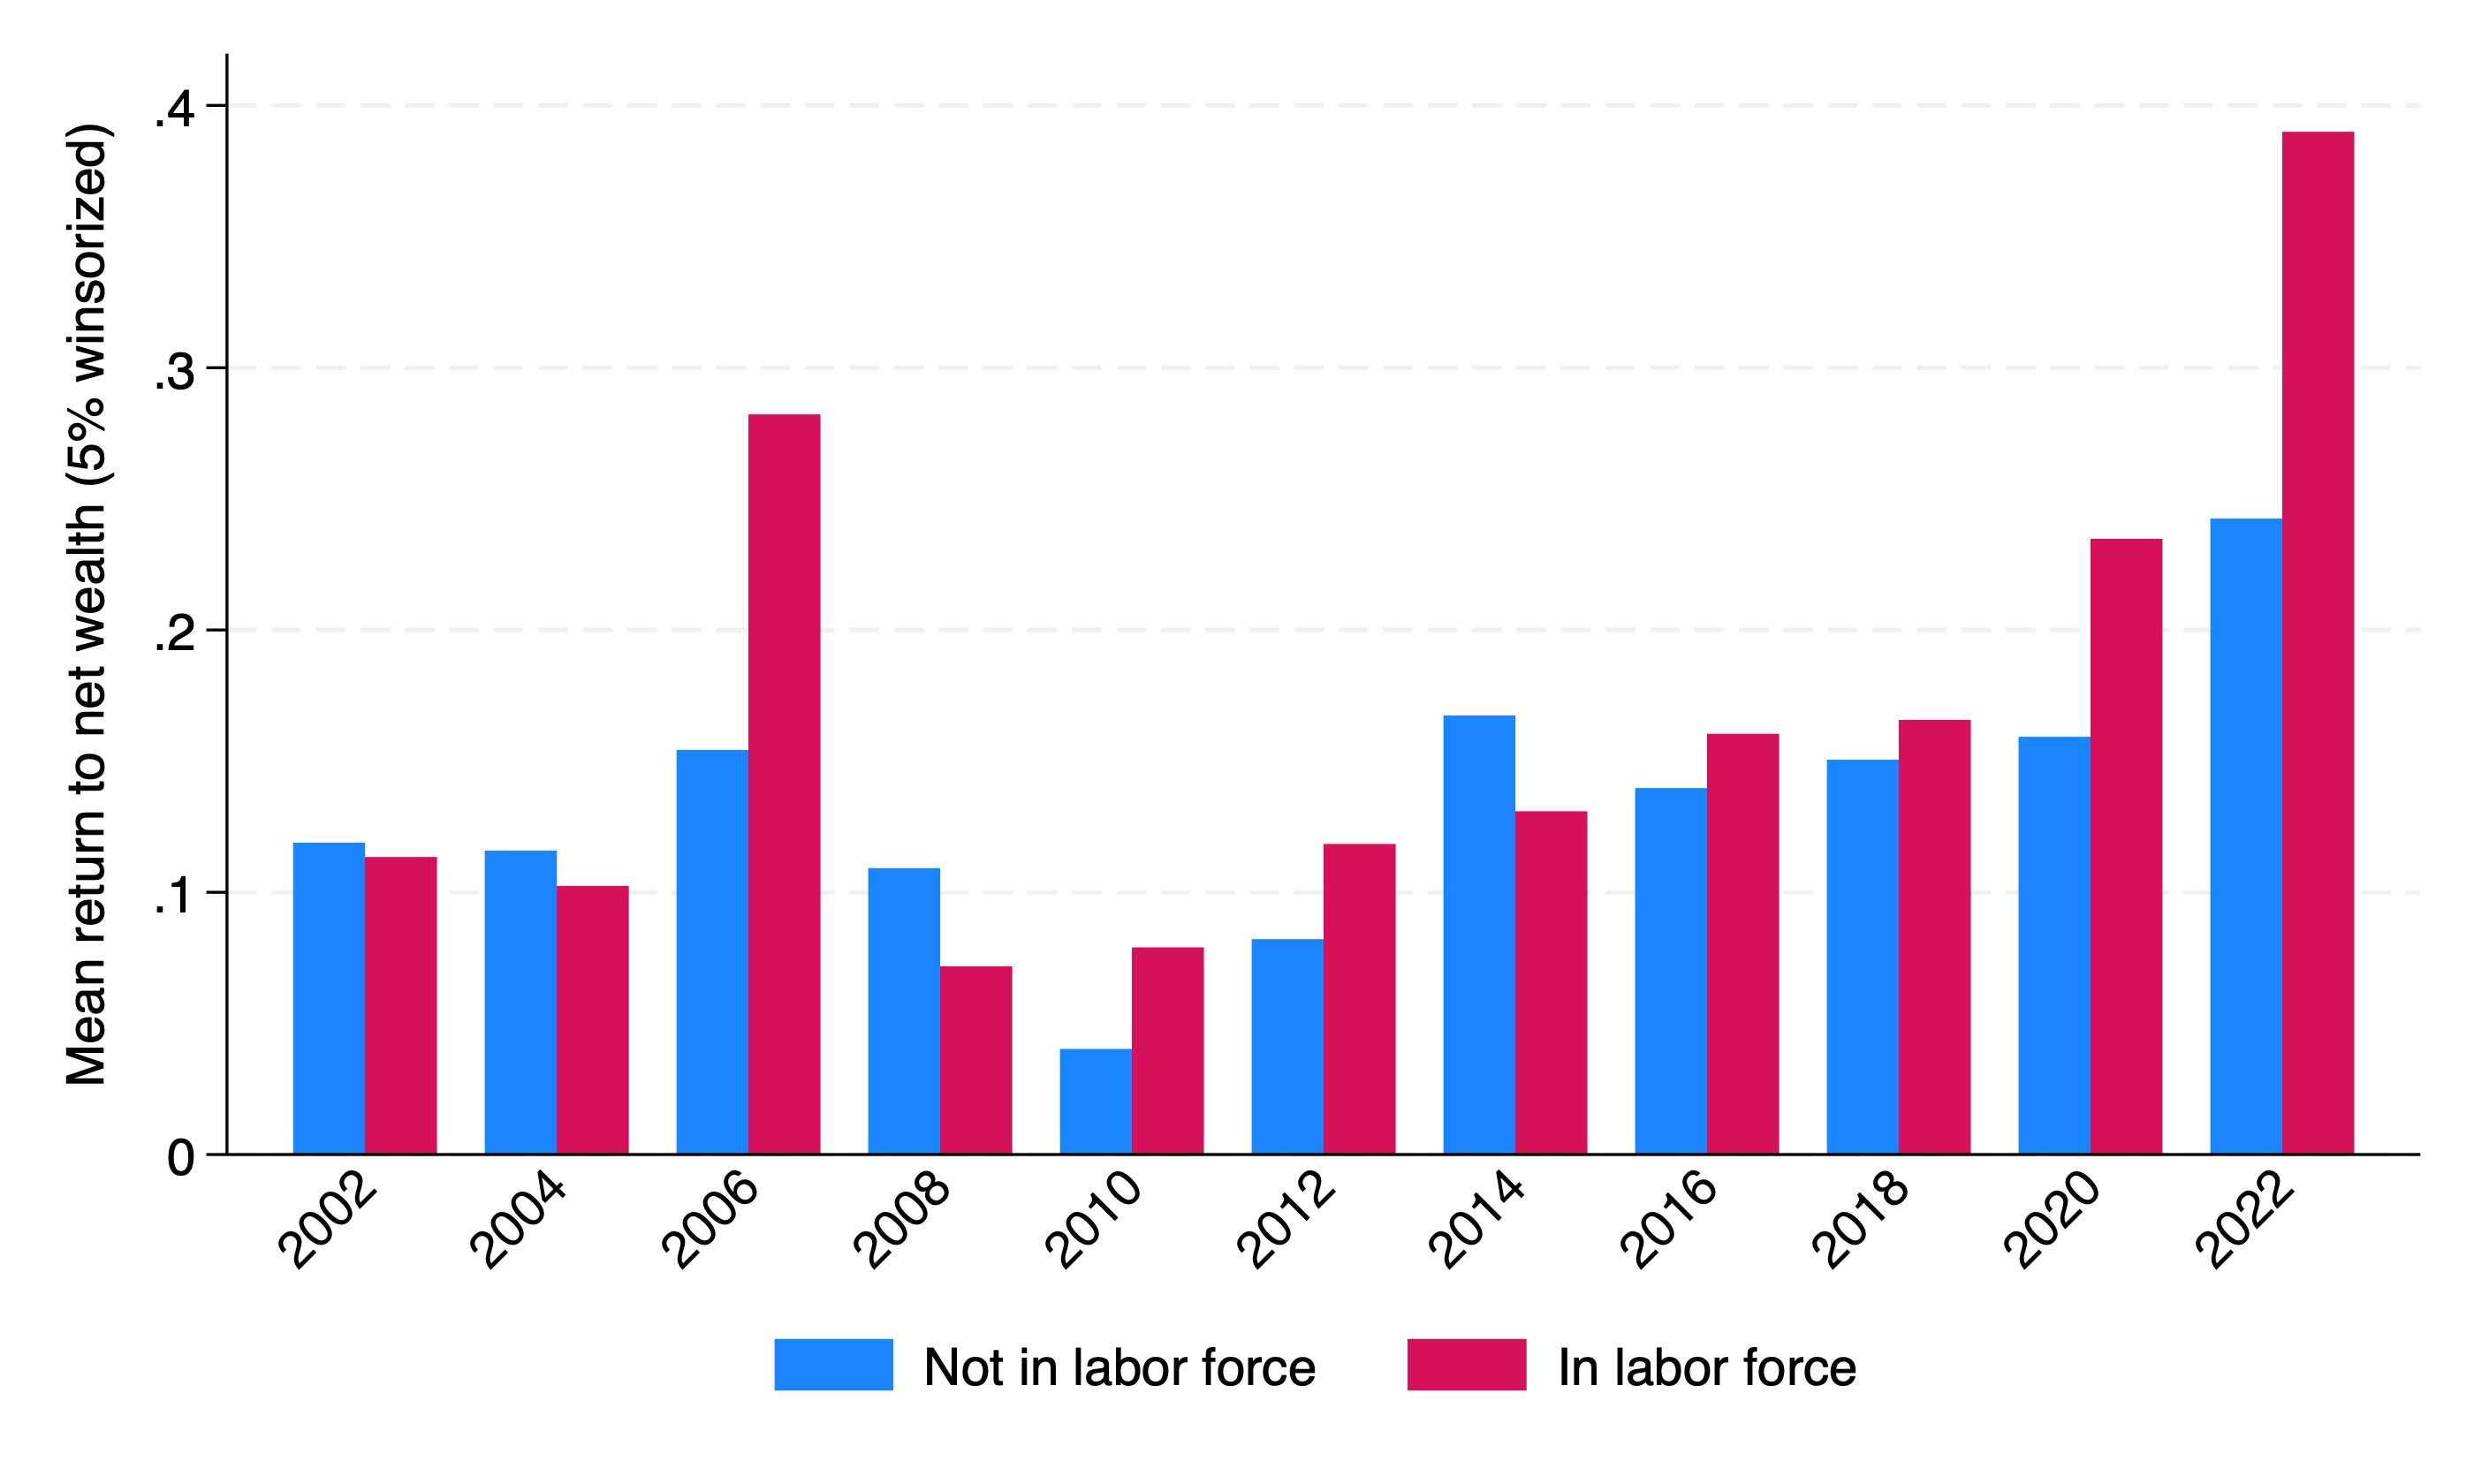
\includegraphics[width=0.85\textwidth]{../../Code/Descriptive/Figures/39_pooled_r5_mean_by_year_inlbrf.png}
\caption{Average returns to net wealth conditional on \texttt{Labor Force Status}}
\label{fig:39_r5_lf_year}
\end{figure}
\FloatBarrier

\subsection{Trust and returns to net wealth}

\par Establishing an empirical relationship between trust and returns is a major goal of this paper. To begin in this direction, I inspect the relationship between trust responses and computed returns to net wealth values for the sample. Figure~\ref{fig:39_r5_vs_trust} suggests some evidence of a hump-shaped relationship between trust and returns to net wealth, as the highest return values seem to be concentrated at the moderate trust ranges.

\begin{figure}[H]
\centering
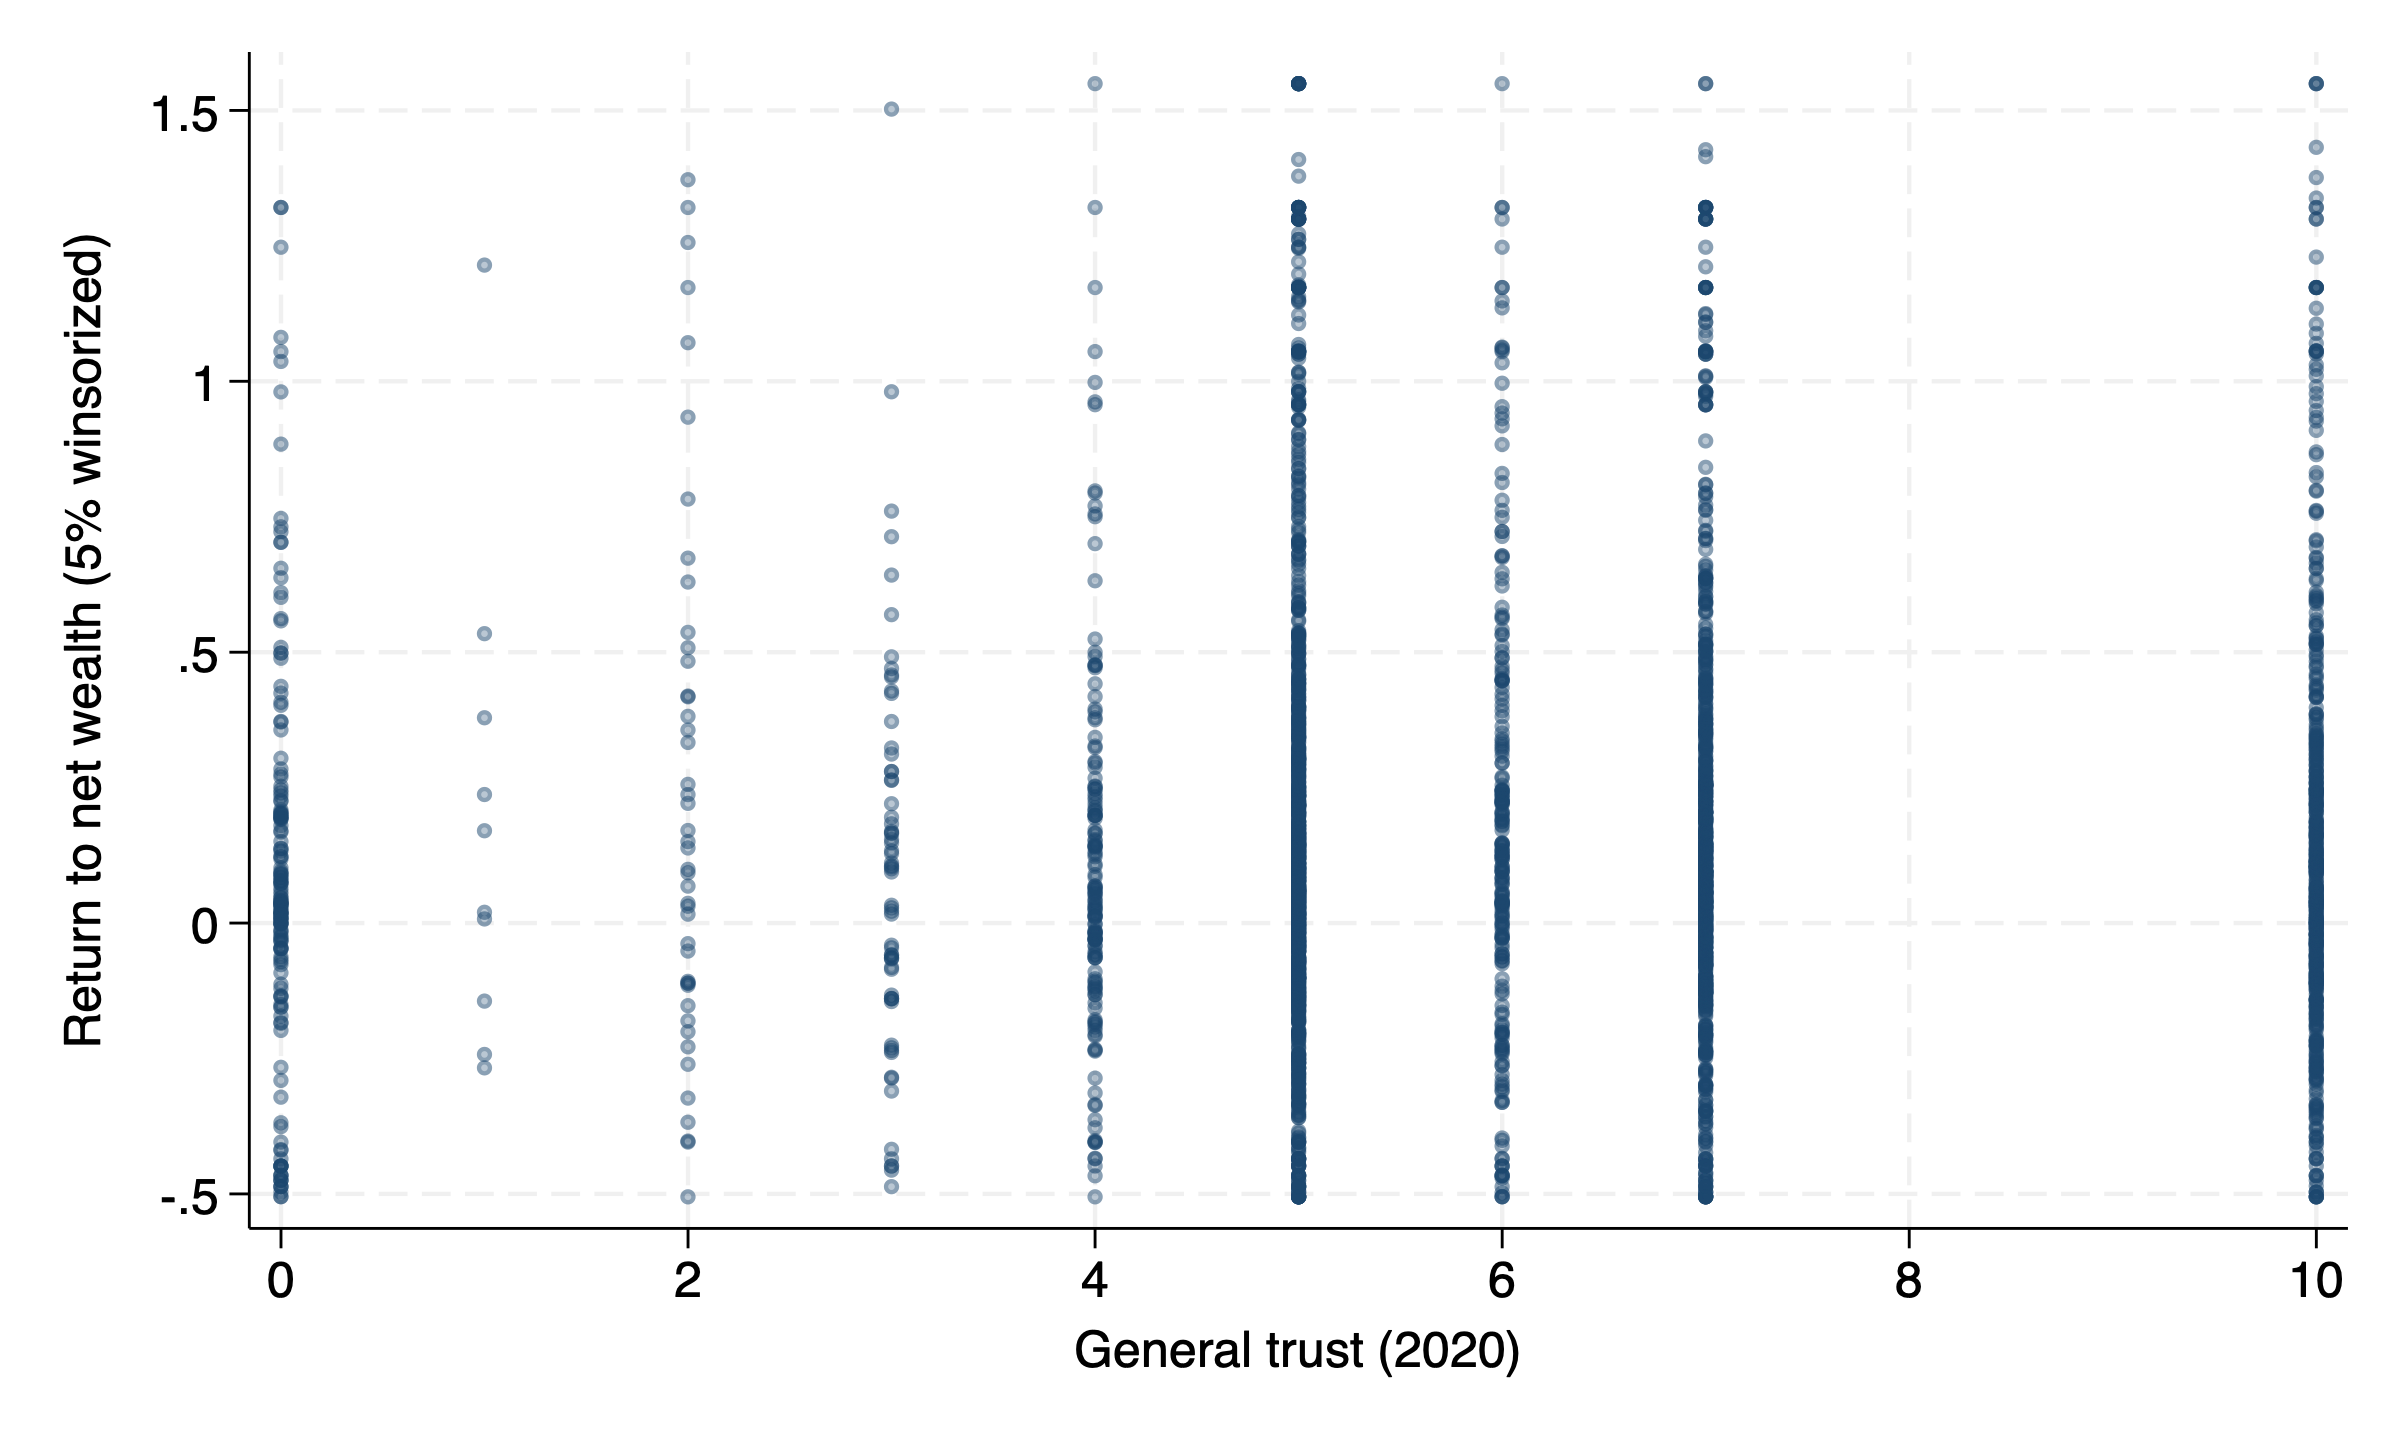
\includegraphics[width=0.8\textwidth]{../../Code/Descriptive/Figures/39_pooled_r5_vs_trust.png}
\caption{Scatterplot of returns to net wealth vs.\ \texttt{Trust}}
\label{fig:39_r5_vs_trust}
\end{figure}
\FloatBarrier

\subsection{Portfolio composition}

\par Table~\ref{tab:41_summary_portfolios} shows that participation is highest in safe assets, residential assets, and the broader core-asset grouping, while direct participation in business and other real estate is much less common. In terms of composition, residential assets account for the largest average share of household balance sheets, followed by core assets and then retirement assets. Debt is also economically important in the pooled sample: over half of person-years involve some debt, and the leverage measures show a long right tail, especially for long-term and total debt.

\InputStataRegTableCompact{\textbf{Participation and Portfolio Composition}}{tab:41_summary_portfolios}{../../Code/Analysis/Tables/41_table5_summary_portfolios.tex}{All shares are expressed as fractions of gross wealth. Participation is the fraction of person-years with a strictly positive holding. Person-years match the pooled regression sample used for Tables~\ref{tab:39_r5_age_bin} and~\ref{tab:39_r5_educ_cat}. Leverage ratios can exceed one when liabilities exceed gross assets. Person-year observations per statistic range from 2{,}886 to 2{,}886 (same pooled regression sample as return descriptives by age and education). The modest spread reflects missing values for specific portfolio components in some person-years.
}
\FloatBarrier

\par Table~\ref{tab:41_asset_shares_by_wealth} shows that asset composition shifts sharply across the wealth distribution. At the bottom, balance sheets are dominated by debt, with very little exposure to business, stocks, or other real estate. Moving up the distribution, risky assets become more important: stocks, business wealth, and other real estate all rise with wealth, and at the very top business ownership becomes especially prominent. This is consistent with the idea that observed portfolio exposure is highly heterogeneous across households.

\InputStataRegTableCompact{\textbf{Asset and Debt Composition by Core Wealth Fractiles}}{tab:41_asset_shares_by_wealth}{../../Code/Analysis/Tables/41_table6_asset_shares_by_wealth.tex}{Mean share of gross wealth in core assets in each of the asset/liability classes, computed as fractile of the core wealth distribution. Fractile boundaries use rank within the same pooled regression person-year sample as Tables~\ref{tab:39_r5_age_bin} and~\ref{tab:39_r5_educ_cat}. Safe assets $=$ bonds + checking/saving.}
\FloatBarrier

\par The broader portfolio aggregates in Table~\ref{tab:41_port_shares_by_wealth} tell a similar story. Residential wealth is the dominant asset for much of the middle of the distribution, while core assets take over at the top, and retirement assets are largest in the upper-middle and upper-tail groups rather than at the very top. Debt shares fall rapidly with wealth, so leverage is concentrated in the lower part of the distribution.


\InputStataRegTableCompact{\textbf{Asset Class Composition by Net-Wealth Fractiles}}{tab:41_port_shares_by_wealth}{../../Code/Analysis/Tables/41_table7_port_shares_by_wealth.tex}{Mean share of gross wealth in each broad asset/liability class, computed within net-wealth fractiles for the same pooled regression person-year sample as Tables~\ref{tab:39_r5_age_bin} and~\ref{tab:39_r5_educ_cat}. Core $=$ business + stocks + bonds + checking/savings + other real estate. Total debt $=$ long-term debt + other debt.}
\FloatBarrier

\par These composition patterns matter in Section~\ref{sec:exts}, where I revisit the main specifications by using the portfolio shares as a proxy for risk exposure.
